\documentclass[9pt, preprint]{sigplanconf} % <<<

% Keep fontenc and inputenc them in this order.
\usepackage[T1]{fontenc}
\usepackage[latin1]{inputenc}

\usepackage{amsmath}
\usepackage{amssymb}
\usepackage{amsthm}
\usepackage{booktabs}
\usepackage{graphics}
\usepackage{microtype}  % do not remove
\usepackage{multirow}
\usepackage{proof}
\usepackage{pygmentize}
\usepackage{rgalg}
\usepackage{tikz}
\usepackage{xcolor}
\usepackage{xspace}

\usepackage{tikz}
\usetikzlibrary{arrows,positioning,fit,backgrounds,shadows,calc}

\usepackage[colorlinks]{hyperref} % keep it last to avoid some warnings

\RecustomVerbatimEnvironment{Verbatim}{BVerbatim}{}
\definecolor{darkred}{rgb}{0.4,0,0}
\definecolor{darkblue}{rgb}{0,0,0.4}
\definecolor{verylightgray}{rgb}{0.9,0.9,0.9}
\definecolor{lightblue}{rgb}{0,0,0.9}
% comment the next line for printing
\hypersetup{colorlinks,linkcolor=darkblue,citecolor=darkblue,urlcolor=darkblue}
\hypersetup{
  pdftitle={Runtime Verification Based on Register Automata},
  pdfauthor={Radu Grigore and Dino Distefano and Rasmus Lechedahl Petersen}}

\title{Runtime Verification Based on Register Automata}
\authorinfo{Radu Grigore}
           {Queen Mary, University of London}
           {rgrig@eecs.qmul.ac.uk}
\authorinfo{Dino Distefano}
           {Queen Mary, University of London}
           {ddino@eecs.qmul.ac.uk}
\authorinfo{Rasmus Lerchedahl Petersen}
           {Microsoft Research}
           {a-rapete@microsoft.com}
\authorinfo{Nikos Tzevelekos}
           {Queen Mary, University of London}
           {nikost@eecs.qmul.ac.uk}


\renewcommand{\sectionautorefname}{Section}
\renewcommand{\subsectionautorefname}{\sectionautorefname}

\newcommand{\noterg}[2]{\textcolor{gray}{[\textcolor{red}{#1}: #2]}}
\newcommand{\rg}[1]{\noterg{rg}{#1}}
\newcommand{\rlp}[1]{\noterg{rlp}{#1}}
\newcommand{\dd}[1]{\noterg{dd}{#1}}
\newcommand{\dinocomment}[1]{\dd{#1}}

\newcommand{\B}{\ensuremath{\mathbb{B}}}
\newcommand{\N}{\ensuremath{\mathbb{N}}}
\newcommand{\delimitVerbatim}{\par\nobreak\smallskip\noindent}
\newcommand{\error}{\ensuremath{\textcolor{darkred}{\mathtt{error}}}\xspace}
\newcommand{\eval}[1]{[[#1]]}
\newcommand{\limp}{\Rightarrow}
\newcommand{\pattern}[1]{\ensuremath{\mathtt{\underline{#1}}}}
\newcommand{\pmap}{\rightharpoonup}
\newcommand{\set}[1]{\ensuremath{\mathsf{#1}}}
\newcommand{\start}{\ensuremath{\mathtt{start}}\xspace}
\newcommand{\verbline}[2][]{\[\text{\Verb@#2@}#1\]}

\newcommand{\quoteindent}{1.5\parindent} % could be re-defined before a quote
\newcommand{\eqquote}[2]{{%
  \refstepcounter{equation}\label{#2}%
  \newdimen\qi\qi=\quoteindent
  \setbox0=\vbox{\advance\hsize by-2\qi\noindent\em#1}%
  \newdimen\x\x=\ht0 \advance\x by\dp0%
  \setbox1=\vbox to\x{\vss\hbox{(\arabic{equation})}\vss}%
  \leavevmode\\[1ex]%
  \hbox to\hsize{\hskip\qi\box0\hfil\box1}%
  \\[1ex]}}
\newcommand{\emquote}[1]{{%
  \\[1ex]%
  \newdimen\qi\qi=\quoteindent%
  \hbox to\hsize{\hfil\vbox{\advance\hsize by-2\qi\noindent\em#1}\hfil}%
  \\[1ex]}}

% rg: I tend to give grammars in BFS order
\def\grammar#1{{
  \footnotesize
  \def\b##1{{\rm\Verb@##1@}}\def\*{$^*$}\def\?{$^?$}\def\({$($}\def\){$)$}
  \def\|{$\mid$}\def\+{$^+$}
  \smallskip
  \hbox to\hsize{\hfil\vbox{\halign{\hfil\it##&$\;::=\;$\it##\hfil&\qquad\rm##\hfil\cr#1}}\hfil}
  \smallskip
}}


\newtheorem{lemma}{Lemma}
\providecommand*{\lemmaautorefname}{Lemma}
\newtheorem{proposition}{Proposition}
\newtheorem{theorem}{Theorem}

\theoremstyle{definition}
\newtheorem{definition}{Definition}
\providecommand*{\definitionautorefname}{Definition}
\newtheorem{example}{Example}
\providecommand*{\exampleautorefname}{Example}

\theoremstyle{remark}
\newtheorem{notation}{Notation}
\newtheorem{remark}{Remark}

% For the final version, switch then comment-status of the following lines.
\overfullrule=5pt
%\renewcommand{\noterg}[2]{}

\showboxdepth=10
\showboxbreadth=30
% >>>
\begin{document}
\maketitle
\begin{abstract} % <<<
We introduce a new formal framework aimed at checking temporal safety properties of object-oriented programs.
The underpinning theoretical foundations of our framework is an extended class of {\em register automata}.
As registers' value can be updated, our automata are able to express highly complex properties of systems involving multiple interacting objects.
Specifications are then used to instrument Java bytecode so that their violations can be automatically detected at runtime.
The precision of the monitoring system is tunable by means of a parameter.
We have validated our technique by checking several safety properties on large open source projects.

\end{abstract}

% >>>
\section{Introduction} % <<<

Runtime verification is a technique where the behaviour of programs is monitored at runtime to check whether executions
can violate certain safety properties.
Systems for runtime verification stand somehow in between classic verification and testing: they work on the actual system (as testing) but check violations of temporal properties as, for example, it is done in model checking. Compared to traditional formal verification techniques, runtime verification systems check only certain program executions, however, the error reports are accurate and detected violations represent real bugs in the program.

In the context of object-oriented programming  leading runtime verification techniques include JavaMOP~\cite{dblp:journals/sttt/meredithjgcr12}, QVM~\cite{arnold:2008}, Tracematches~\cite{dblp:conf/oopsla/allanachklmsst05}, and techniques based on typestate~\cite{strom1986,dblp:conf/oopsla/bierhoffa07,dblp:conf/oopsla/naeeml08,disney2011,ball2002}. Although powerful,  these methods present some limitations. For example, either   in terms of  language expressivity, or in the ability to express concisely properties of the interaction of several objects 
over time (typestate), or in concisely expressing  properties requiring an unbounded number of different object re-bidings (sometimes called "parameters" in the runtime verification community).

Register Automata~\cite{dblp:conf/focs/kaminskif90} are automata where a number of registers are used to store and compare data. Value of registers can be updated overtime, and  data can be taken from unbounded domains (e.g., the set of object references). Thus register automata provide a powerful device for reasoning about temporal 
relations of a (possibly unbounded) number of objects in a finite manner. They have been studied extensively from the theoretical point of
view and essential results for their analysis have been established (e.g., decidability of emptyness, closure under intersection, and so forth).

Thus, it seems sensible to attempt an approach to runtime verification taking register automata as starting point. The aim is to
exploit the flexibility and the power of registers to
address certain properties not easily dealt with in other approaches.
On the formal side, we started from register automata and have extended them driven by typical properties required in real-world object-oriented systems.
The extension has been careful crafted to be able to define the precise mathematical connection with register automata, and yet,
make it easy for programmers to express properties of their code. This process has resulted in the definition of two new classes of 
automata: a high-level and a low-level one. In the high-level automata, temporal properties about programs are naturally expressed. Low-level automata, 
on the other hand, simplify the formal correspondence with  register automata. 
Finally we defined a formal language --- called TOPL (Temporal Object Property Language) --- mapping directly on the 
high-level automata.

We complement the theoretical construction with a practical tool.
We have implemented TOPL  in a runtime parametric verification framework that can be used by Java programmer to express rigorous temporal 
properties about their programs. These properties will be then automatically checked by the system.
The formal correspondence between the properties and register automata defined in this paper gives rigorous mathematical foundation to
the approach and allow us to reuse many of the results for register automata on TOPL automata. For example, given a TOPL property, we can statically analyse whether its language is empty.  The formal development is completely hidden from 
the programmer.  Thus TOPL provides developers with a flexible methodology for enforcing safety constraints on their code.
Our system can be tuned  in terms of coverage,  overhead, and trace reporting by means of a numerical parameter. 


%For example, every iterator and every collection in \texttt{java.util} contains checks concerning the example property~\eqref{q:concur-it}.
%It is impossible to turn off these checks, even if one has a proof that a certain program correctly uses the library.
%Because these checks are always active, their overhead must be very low.
%As a result, when a check fails, the user is not provided with an error trace.
%Also, such checks are difficult to write and to maintain. Other libraries document such temporal constraints only in (informal) comments.
%With TOPL, the programmer (formally) describes the properties in one place, which is separate from the code. 
%This description serves as a rigorous documentation (because of the formal semantics) of which safety properties are enforced on the program.
%Then it is the job of the TOPL compiler to insert the appropriate checks into the Java bytecode of the program.
%The execution is monitored and violations are reported as traces of events.
%The programmer has the ability to tune the overhead by choosing how many objects to track, for how long to remember past events, and a few other parameters. For example, during testing they could allow for a very high overhead, whereas they could choose to deploy the bytecode without any inserted check.

\paragraph{Contributions.}
In summary, the contributions of this paper are:\dd{add the rtopl-->topl}
\begin{itemize}
\item We define TOPL, a formal specification language tailored to express properties involving object interactions over time in a way that is familiar to object-oriented programmers.
\item We define a precise formal semantics for TOPL, making it suitable for program analysis, both static and dynamic.
\item We define a precise formal correspondence between TOPL automata and register automata. This allows us to check several characteristic of TOPL specifications (e.g., the non-emptiness of their language).
\item We have implemented our parametric framework  in a tool that automatically check at runtime violations of TOPL properties in Java programs. A numerical parameter is used to tune the precision of the system.

\item We report the experimental results of running our tool on large open-source projects. The results are encouraging: we have found
violations of properties, and we have observed an acceptable runtime overhead. 
\end{itemize}


The paper is organized as follows.\dinocomment{fix at the end}
\autoref{sec:results} gives the experimental results.
\autoref{sec:examples} introduces the TOPL language with examples.
\autoref{sec:implementation} describes a the interesting aspects of the implementation.
\autoref{sec:related} discusses related work.
Finally, \autoref{sec:conclusions} concludes the paper and describes our plans for future work.

%>>>
\section{Motivating Examples} %<<<
Interaction among objects is at the core of the object-oriented paradigm.
Consider the classes in Figure~\ref{fig:first.java}.
Class {\tt CharArray} manipulates an array of chars and implements the {\tt Str} interface. 
Class {\tt Concat} is used to concatenate two object of type {\tt Str}. The concatenation implements also the
 {\tt Str} interface.

A typical property one would want to state for a program using these classes (as well as Java collections in general) is:
\eqquote{If one iterator modifies its collection, then other existing iterators of the same collection become invalid, which means they cannot be used further.}{q:concur-it}
The formalization of the above constraint is non-trivial since it needs to keep track of {\em several objects} (at least two iterators, and one collection), their {\em interaction over time}, and possible {\em variable updates}.
\begin{figure}[t] % first example <<<
%\begin{Verbatim}[commandchars=\\\{\}]
\PY{k+kn}{import} \PY{n+nn}{java.util.*}\PY{o}{;}
\PY{k+kd}{public} \PY{k+kd}{class} \PY{n+nc}{IncorrectIteratorUse} \PY{o}{\PYZob{}}
  \PY{k+kd}{public} \PY{k+kd}{static} \PY{k+kt}{void} \PY{n+nf}{main}\PY{o}{(}\PY{n}{String}\PY{o}{[}\PY{o}{]} \PY{n}{args}\PY{o}{)} \PY{o}{\PYZob{}}
    \PY{n}{List}\PY{o}{<}\PY{n}{Integer}\PY{o}{>} \PY{n}{c} \PY{o}{=} \PY{k}{new} \PY{n}{ArrayList}\PY{o}{<}\PY{n}{Integer}\PY{o}{>}\PY{o}{(}\PY{o}{)}\PY{o}{;}
    \PY{n}{c}\PY{o}{.}\PY{n+na}{add}\PY{o}{(}\PY{l+m+mi}{1}\PY{o}{)}\PY{o}{;} \PY{n}{c}\PY{o}{.}\PY{n+na}{add}\PY{o}{(}\PY{l+m+mi}{2}\PY{o}{)}\PY{o}{;}
    \PY{n}{Iterator}\PY{o}{<}\PY{n}{Integer}\PY{o}{>} \PY{n}{i} \PY{o}{=} \PY{n}{c}\PY{o}{.}\PY{n+na}{iterator}\PY{o}{(}\PY{o}{)}\PY{o}{;}
    \PY{n}{Iterator}\PY{o}{<}\PY{n}{Integer}\PY{o}{>} \PY{n}{j} \PY{o}{=} \PY{n}{c}\PY{o}{.}\PY{n+na}{iterator}\PY{o}{(}\PY{o}{)}\PY{o}{;}
    \PY{n}{i}\PY{o}{.}\PY{n+na}{next}\PY{o}{(}\PY{o}{)}\PY{o}{;} \PY{n}{i}\PY{o}{.}\PY{n+na}{remove}\PY{o}{(}\PY{o}{)}\PY{o}{;} \PY{n}{j}\PY{o}{.}\PY{n+na}{next}\PY{o}{(}\PY{o}{)}\PY{o}{;}
  \PY{o}{\PYZcb{}}
\PY{o}{\PYZcb{}}
\end{Verbatim}

\begin{tiny}
\begin{Verbatim}[commandchars=\\\{\}]
\PY{k+kd}{interface} \PY{n+nc}{Str} \PY{o}{\PYZob{}}
  \PY{k+kt}{void} \PY{n+nf}{set}\PY{o}{(}\PY{k+kt}{int} \PY{n}{i}\PY{o}{,} \PY{k+kt}{char} \PY{n}{c}\PY{o}{)}\PY{o}{;}  \PY{k+kt}{char} \PY{n}{get}\PY{o}{(}\PY{k+kt}{int} \PY{n}{i}\PY{o}{)}\PY{o}{;}
  \PY{k+kt}{int} \PY{n+nf}{len}\PY{o}{(}\PY{o}{)}\PY{o}{;}
  \PY{n}{Itr} \PY{n+nf}{itr}\PY{o}{(}\PY{o}{)}\PY{o}{;}
\PY{o}{\PYZcb{}}
\PY{k+kd}{interface} \PY{n+nc}{Itr} \PY{o}{\PYZob{}}
  \PY{k+kt}{boolean} \PY{n+nf}{hasNext}\PY{o}{(}\PY{o}{)}\PY{o}{;}        \PY{k+kt}{char} \PY{n}{next}\PY{o}{(}\PY{o}{)}\PY{o}{;}
  \PY{k+kt}{void} \PY{n+nf}{set}\PY{o}{(}\PY{k+kt}{char} \PY{n}{c}\PY{o}{)}\PY{o}{;} 
\PY{o}{\PYZcb{}}
\PY{k+kd}{class} \PY{n+nc}{CharArray} \PY{k+kd}{implements} \PY{n}{Str} \PY{o}{\PYZob{}}
  \PY{k+kt}{char} \PY{o}{[}\PY{o}{]} \PY{n}{data}\PY{o}{;}
  \PY{c+c1}{// ...}
\PY{o}{\PYZcb{}}
\PY{k+kd}{class} \PY{n+nc}{Concat} \PY{k+kd}{implements} \PY{n}{Str} \PY{o}{\PYZob{}}
  \PY{n}{Str} \PY{n}{one}\PY{o}{,} \PY{n}{two}\PY{o}{;}
  \PY{k+kd}{public} \PY{k+kd}{static} \PY{n}{Concat} \PY{n+nf}{make}\PY{o}{(}\PY{n}{Str} \PY{n}{one}\PY{o}{,} \PY{n}{Str} \PY{n}{two}\PY{o}{)} \PY{o}{\PYZob{}} \PY{c+cm}{/* ... */} \PY{o}{\PYZcb{}}
  \PY{c+c1}{// ...}
\PY{o}{\PYZcb{}}
\end{Verbatim}

\end{tiny}
\caption{A first example: Java code}
\label{fig:first.java}
\end{figure}
%The program in \autoref{fig:first.java}. The last statement violates the property of the introduction, therefore throwing an exception.
%There are two iterators on the same collection, one of them modifies the collection, and this invalidates the other iterator.
%To understand the need for keeping track of variables updates, consider the following snippet of code
%\begin{verbatim}
% ....
% i=s.itr();
% .....
% while (ch.more_input()) {
%   CharArray c = ch.get_input();
%   s = Concat(s,c);
% }
%\end{verbatim}
%where strings are read  from an input channel and accumulated in the {\tt Concat} object {\tt s}.
To understand the need for variable updates in the specification, consider the case where 
{\tt Concat} is used to implement a  {\em rope} data structure.\footnote{ A rope is a binary tree shaped data structure for efficiently storing and manipulating very long strings~\cite{DBLP:journals/spe/BoehmAP95}.} 
Rope's operations like insert, concat, delete may update the shape of the tree and references to its root. 
In a temporal specification we would then need either different logical variable for the different values of the root or
the ability to re-bound variable in the temporal specification. 
As  number of the operations on the rope is not known, and  in general can be unbounded, re-binding specification variables with
different values during the computation allows to keep the specification finite. 

\paragraph{Data Structures Shapes.}
One interesting kind of properties for object-oriented programs is the ability to reason about the evolving shape of the heap composed by the allocated objects.
\emquote{The shape of the list should not become neither circular nor pan-handle.}
This is useful for example when we traverse a loop like the following
\begin{verbatim}
  while (l.next()!=null) {
     ......
  }
\end{verbatim}
as a circular/pan-handle list would cause non-termination. Also for encoding properties of this kind it is necessary to be able to update the 
value of the specification variables.

%The following TOPL properties test the shape of a linked list and
%reports an error if it is cyclic or it has the pan-handle shape (i.e.,
%there is a lasso at some point). 
%Directives are omitted.
%%
%\delimitVerbatim
%\begin{Verbatim}[commandchars=\\\{\}]
% property ListNotCyclic
%   start -> start: *
%   start -> a: \pattern{X} := *.getList()
%   a -> a:     \pattern{X} := x.next()
%   a -> b:     \pattern{Y} := x.next()
%   b -> b:     \pattern{Y} := y.next()
%   b -> error: x := y.next()
%   a -> error: x := x.next()
%\end{Verbatim}
%\delimitVerbatim
%The idea is that this property will bind the automaton variable $x$ with any possible object in the list, and the $y$ with any possible successors (via the next field) of the current binding of $x$.
%Therefore, if there is a lasso, in the list, this will be detected when a new biding of $y$ via a \texttt{b -> b} becomes equal to the binding of $x$.
%The transition \texttt{a ->error} detect the case where there is an object pointing to itself.

%
%The following property detects when a dictionary overwrite one of its bindings.
%\delimitVerbatim
%\begin{Verbatim}[commandchars=\\\{\}]
% property BadDictionary
%   message "dictionary overwrites its bindings"
%   observe <Dictionary.*>
%   prefix <Dictionary>
%   start -> start: *
%   start -> written:   \pattern{D}.put(\pattern{K}, \pattern{V})
%   written -> written: d.put(k, \pattern{V})
%   written -> error:   !v := d.get(k)
%\end{Verbatim}
%\delimitVerbatim
%The overwrite is detected by the guard which checks if the value associated with a key $k$ is the same as the original binding recorded in the automaton variable $v$.

% >>>
% >>>
\section{Overview and Background}\label{sec:overview} % <<<

\autoref{fig:concepts} shows the main concepts of concern.
Register automata are well-studied devices, introduced decades ago.
The gap between TOPL properties and register automata is filled by two semantic models, namely high-level and low-level TOPL automata.
The high-level model (rollback TOPL automata) is better suited for implementation;
the low-level model (simple TOPL automata) is easier to analyze.

The target of an arrow is at least as expressive as its source.
All three automata models have the same expressivity.
In general, decision problems on automata (such as membership, emptiness, language inclusion), are either decidable for all three models, or undecidable for all three models.
However, decidable problems do not necessarily have the same complexity for the three models.

\begin{figure}[th]\centering
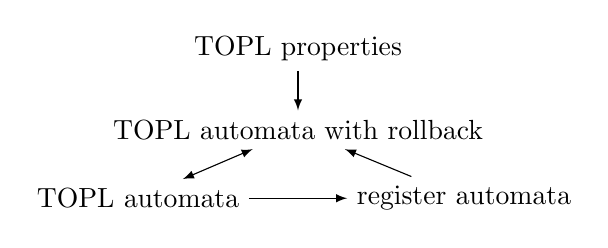
\begin{tikzpicture}[auto,node distance=5mm]
  \node (lang) {TOPL properties};
  \node (rtopl) [below=of lang] {TOPL automata with rollback};
  \node (x) [below=of rtopl] {};
  \node (topl) [left=of x] {TOPL automata};
  \node (ra) [right=of x] {register automata};
  \path[draw,->,>=latex]
    (lang) edge (rtopl)
    (rtopl) edge[<->] (topl)
    (topl) edge (ra)
    (ra) edge (rtopl);
\end{tikzpicture}
\caption{Main concepts}
\label{fig:concepts}
\end{figure}

We review here register automata and several results about them.
Together with the reductions presented later, these results imply similar results about TOPL automata.

We begin by defining a generic automaton, of which both TOPL and register automata are instances.
A \emph{letter} $\ell$ is an $n$-tuple $(v_1,\ldots,v_n)$ of \emph{values} from a possibly infinite set~$V$;
we denote the \emph{alphabet} by~$\Sigma=V^n$.
A \emph{store} $s$ is an $m$-tuple $(u_1,\ldots,u_m)$ of values;
we denote the set of stores by $S=V^m$.
A \emph{register} $i$ is an integer that identifies a component of the store;
the set of registers is $[m]=\{1,2,\ldots,m\}$.
A \emph{guard} $g$ is a formula in some logic interpreted over pairs of letters and stores;
we write $(s,\ell)\models g$ to denote that store $s\in S$ and the letter $\ell\in\Sigma$ satisfy the guard~$g$, and we denote the set of guards by~$G$.
An \emph{action} $a$ is a small program acting on stores, which has relational semantics;
we denote the set of actions by $A=\Sigma\to(S\times S)$.
Thus, an action applied to a letter $a(\ell)$ is a relation on stores.
We will later specialize to specific and simple logics (for guards) and programming languages (for actions).
A \emph{label} $\lambda$ is a pair $(g,a)$ of a guard~$g$ and an action~$a$;
we denote the set of labels by $\Lambda=G\times A$.

\begin{definition}\label{def:automaton}
An \emph{automaton}~${\cal A}$ with $m$~registers over $n$-tuples of values from the set~$V$ consists of
\begin{itemize}
\item a finite set~$Q$ of states
\item an initial state $q_0\in Q$
\item an initial store $s_0\in S$
\item a set $F\subseteq Q$ of final states
\item a finite transition relation $\delta\subseteq Q\times\Lambda\times Q$
\end{itemize}
\end{definition}

A \emph{configuration}~$x$ is a pair~$(q,s)$ of a state~$q$ and a store~$s$;
we denote the set of configurations by $X=Q\times S$.
The \emph{initial} configuration is $(q_0,s_0)$.
A configuration is \emph{final} when its state is final.
The configuration graph of the automaton is a subset of $X\times\Sigma\times X$.
We write \[x_1\stackrel{\ell}{\to}_{\cal A}x_2\] to mean that $(x_1,\ell,x_2)$ is in the configuration graph of~${\cal A}$.
If the automaton is clear from the context, we omit the subscript.

\begin{definition}\label{def:cgraph}
The \emph{configuration graph} of an automaton consists of exactly those configuration transitions \[ (q_1,\sigma_1) \stackrel{\ell}{\to} (q_2,\sigma_2) \] for which there exists an automaton transition $(q_1,(g,a),q_2)\in\delta$ such that $(\sigma_1,\ell)\models g$ and $(\sigma_1,\sigma_2)\in a(\ell)$.
\end{definition}
An automaton is \emph{nondeterministic} when its configuration graph contains two distinct transitions that have the same source~$x_1$ and are labeled by the same letter~$\ell$:
\[ \text{$x_1\stackrel\ell\to x_2$ and $x_1\stackrel\ell\to x_3$,\quad with $x_2\ne x_3$} \]
Otherwise, the automaton is \emph{deterministic}.

The \emph{language}~${\cal L}({\cal A})$ of an automaton~${\cal A}$ is the set of words that label walks from the initial configuration to some final configuration:
\[ {\cal L}({\cal A}) =
  \{\,\ell_1\ldots\ell_k\mid \text{$x_0$ initial,
  $x_{i-1}\stackrel{\ell_i}\to_{\cal A} x_i$ for $i\in[k]$,
  $x_k$ final}\,\}\]
Being a walk rather than a path, the configurations $x_0$,~$x_1$, \dots,~$x_k$ need not be distinct.

\smallskip

Given a number~$m$ of registers, an arity~$n$ for letters, and a countable set~$V$ of values, the set $A=\Sigma\to(S\times S)$ of actions is uncountable.
Therefore we must focus on a subset of $A$ if we want our automata to be finitely representable.
We will only consider actions that are sequences of assignments.
The assignment $({\sf set}\,i:=j)$ is defined as follows:
\[ \bigl((v_1,\ldots,v_m),(v'_1,\ldots,v'_m)\bigr)\in
  ({\sf set}\,i:=j)\bigl((u_1,\ldots,u_n)\bigr) \]
if and only if $v'_k=v_k$ for all~$k$, except that $v'_i=u_j$.
The sequence operator~$;$ is defined by saying that the relation $(a_1;a_2)(\ell)$ is the composition of the relations $a_1(\ell)$ and $a_2(\ell)$, for all~$\ell$.
The identity action ${\sf nop}$ satisfies ${\sf nop}(\ell)=\{\,(\sigma,\sigma)\mid\sigma\in S\,\}$ for all~$\ell$.

Register automata work with arity $n=1$, that is $\Sigma=V$.
In this case we write $({\sf set}\,i)$ as a shorthand for $({\sf set}\,i:=1)$.
The syntax of guards for register automata is the following:
\begin{align*}
G_{\rm RA} &\;::=\; {\sf fresh} \mid {\sf eq}\,i
\end{align*}
They are interpreted as follows:
\begin{align*}
\bigl((u_1,\ldots,u_m),v\bigr)&\models{\sf fresh}
  &&\text{iff $u_i\ne v$ for all $i$} \\
\bigl((u_1,\ldots,u_m),v\bigr)&\models{\sf eq}\,i
  &&\text{iff $u_i=v$}
\end{align*}

With these notations we can fix a definition for register automata.

\begin{definition}
A \emph{register automaton} with $m$~registers is an automaton over the alphabet $\Sigma=V$ whose labels 
are given by $\Lambda=\bigl\{\,({\sf fresh},{\sf set}\,i),\; ({\sf eq}\,i, {\sf nop})  \mid i\in[m] \,\bigr\}$.
\label{def:ra}
\end{definition}

There are several variants of definitions for register automata in the literature.
%It is even the case that several published results hold only for certain variants of the definition.
Our variant corresponds directly to what Neven et al~\cite{dblp:conf/mfcs/nevensv01} call 1N-RA (for `one-way non-deterministic register automata').

\begin{example}\label{ex:ra1}
The language $\{\,abc\mid\text{$a\ne c$ and $b\ne c$}\,\}$ is recognized by the following register automaton with $3$~registers over the alphabet $\Sigma=V\cup\{\bot\}$:
\begin{itemize}
\item $Q=\{1,2,3,4\}$
  and $q_0=1$
  and $\sigma_0=(\bot,\bot,\bot)$
  and $F=\{4\}$
\item the set of transitions is
\begin{align*}\delta =\{ & \bigl(1,({\sf fresh},{\sf set}\,1),2\bigr), \ \bigl(2,({\sf fresh},{\sf set}\,2),3\bigr), \\
& \bigl(2,({\sf eq}\,1,{\sf nop}),3\bigr), \bigl(3,({\sf fresh},{\sf set}\,1),4\bigr) \}.
\end{align*}
\end{itemize}
Observe that:
(1)~The two parallel transitions from 2~to~3 are needed because labels cannot have the shape $({\sf true},{\sf set}\,i)$; in fact, we have not even defined yet the guard {\sf true}.
(2)~Only values from~$\sigma_0$ may appear multiple times in a store; in this case, only~$\bot$.
(3)~Register~3 ensures that $\bot$ will not appear in the third position of words, which is a risk because we extended the alphabet.
(4)~The action of the last transition is superfluous, but required by the definition.
\end{example}

Let's consider the following  standard decision problems for automata. For an automaton ${\cal A}$,
the membership problem asks whether $w\in {\cal L}({\cal A})$ for a given word~$w$.
The emptiness problem asks whether ${\cal L}({\cal A}) = \emptyset$.
The  universality problem asks whether $w\in{\cal L}({\cal A})$ for all words~$w$.
For automata ${\cal A_1}$ and ${\cal A_2}$, the  language inclusion problem asks whether ${\cal L}({\cal A}_1) \subseteq {\cal L}({\cal A}_2)$.

\begin{theorem}\label{th:ra}
The following properties of register automata are known:
\begin{enumerate}
\item The emptiness problem is coNP-complete~\cite{dblp:journals/tcs/sakamotoi00}.
\item The membership problem is NL-complete~\cite{dblp:conf/mfcs/nevensv01}.
\item The containment, equivalence, and universality problems are decidable for $2$~registers.~\cite{dblp:conf/focs/kaminskif90}
\item The universality, containment, and equivalence problems are undecidable in general~\cite{dblp:conf/mfcs/nevensv01}.
\item Register automata are closed under union, intersection, concatenation, and Kleene star.~\cite{dblp:conf/focs/kaminskif90}
\item Register automata are \emph{not} closed under complementation~\cite{dblp:conf/focs/kaminskif90}.
\item Nondeterministic register automata are strictly more expressive than deterministic register automata~\cite{dblp:conf/focs/kaminskif90}.
\item The language ${\cal L}({\cal A})\cap C^*$ is regular for any register automaton~${\cal A}$ and any finite subset $C\subset V$ of values~\cite{dblp:conf/focs/kaminskif90}.
\end{enumerate}
\end{theorem}

These results have analogues for TOPL automata.
The details depend on what exactly the arrows from \autoref{fig:concepts} are.
The gist will generally be a transformation of the following kind:
From an automaton~${\cal A}$ in one model, construct an automaton~${\cal A}'$ in another model such that
\[ \ell_1\ldots \ell_k \in {\cal L}({\cal A})
  \iff
f(\ell_1)\ldots f(\ell_k)\in{\cal L}({\cal A}') \]
for some fixed $f$ that is easily computable.
The interesting ideas will be in how ${\cal A}'$~is built;
$f$~handles technicalities.

%>>>
\section{TOPL Automata}\label{sec:topl_automata} % <<<

We now gradually move towards a model that is better suited for runtime verification of Java programs.

\subsection{Simple TOPL Automata} %<<<

TOPL automata work with the alphabet $\Sigma=V^n$ for some~$n\in\N$, unlike register automata, which force $n=1$.
It is then natural to consider different guards and actions, which handle specific components of the letters.
TOPL guards are the following:
\begin{align*}
G_{\rm TOPL} &\;::=\; {\sf eq}\,i=j \\
G_{\rm TOPL} &\;::=\; {\sf neq}\,i\ne j \\
G_{\rm TOPL} &\;::=\; {\sf true} \\
G_{\rm TOPL} &\;::=\; G_{\rm TOPL} \mathrel{\sf and} G_{\rm TOPL}
\end{align*}
If $n=1$, we write $({\sf eq}\,i)$ instead of $({\sf eq}\,i=1)$, and $({\sf neq}\,i)$ instead of $({\sf neq}\,i\ne1)$.
These abbreviations are similar to the one used for assignments.
The guards are interpreted as follows:
\begin{align*}
\bigl((u_1,\ldots,u_m),(v_1,\ldots,v_n)\bigr) &\models {\sf eq}\,i=j
  &&\text{iff $u_i=v_j$} \\
\bigl((u_1,\ldots,u_m),(v_1,\ldots,v_n)\bigr) &\models {\sf neq}\,i\ne j
  &&\text{iff $u_i\ne v_j$}
\end{align*}
and
\begin{align*}
(\sigma,\ell) &\models {\sf true}
  &&\text{always} \\
(\sigma,\ell) &\models g_1\mathrel{\sf and} g_2
  &&\text{iff $(\sigma,\ell)\models g_1$ and $(\sigma,\ell)\models g_2$}
\end{align*}

We can now define TOPL automata.

\begin{definition}
A \emph{TOPL automaton} is an automaton whose guards are from the set~$G_{\rm TOPL}$ (defined above) and whose actions are sequences of assignments (defined in \autoref{sec:overview}).
\end{definition}

\begin{example}\label{ex:topl1}
Consider again the language $\{\,abc\mid\text{$a\ne c$ and $b\ne c$}\,\}$.
It is recognized by the following TOPL automaton with $2$~registers over the alphabet $\Sigma=V$:
\begin{itemize}
\item $Q=\{1,2,3,4\}$ and $q_0=1$ and $F=\{4\}$
\item $\delta$ consists of
  $\bigl(1,({\sf true}, {\sf set}\,1),2\bigr)$
  and $\bigl(2,({\sf true}, {\sf set}\,2),3\bigr)$
  and $\bigl(3,({\sf neq}\,1\mathrel{\sf and}{\sf neq}\,2, {\sf nop}),4\bigr)$.
\end{itemize}
Any initial store~$\sigma_0$ works.
\end{example}

Examples \ref{ex:ra1}~and~\ref{ex:topl1} hint that a general  transformation from TOPL automata to register automata is not very easy to find.
We describe an encoding chain ${\cal A}_1\to{\cal A}_2\to{\cal A}_3\to{\cal A}_4$ that goes from a TOPL automaton~${\cal A}_1$ to a register automaton~${\cal A}_4$.
The encoding ${\cal A}_2\to{\cal A}_3$ is more difficult than the other two.

\paragraph{Step ${\cal A}_1\to{\cal A}_2$.}
The automaton~${\cal A}_2$ works over the alphabet~$V$, while ${\cal A}_1$ may work on an alphabet~$V^n$ with $n>1$.
The number of registers is preserved.
Each letter $(v_1,\ldots,v_n)$ is transformed into the word $v_1\ldots v_n$ repeated $m+1$ times.
Each transition $\bigl(q_1,(g,a),q_2\bigr)$ is encoded with a path from~$q_1$ to~$q_2$ of length $(m+1)n$.
The first $n$~transitions encode the guard~$g$ -- they are labeled $(g_1,{\sf nop})$, \dots, $(g_n,{\sf nop})$.
The guard~$g_j$ contains the conjunct ${\sf eq}\,i$ if and only if $g$~contains the conjunct ${\sf eq}\,i=j$; similarly for ${\sf neq}$.
The following $mn$~transitions encode the action~$a$ -- they are labeled $({\sf true}, a_1)$, \dots, $({\sf true}, a_{mn})$.
If the last assignment of~$a$ to register~$i$ is ${\sf set}\,i:=j$, then $a_{(i-1)m+j}$ is ${\sf set}\,i$.
Otherwise, if $a$ does not assign at all to register~$i$, then $a_{(i-1)m+1}$ is ${\sf nop}$.

The labels of~${\cal A}_2$ have one of the following shapes:
\begin{itemize}
\item $({\sf eq}\,i_1\mathrel{\sf and}{\sf eq}\,i_2\ldots
  \mathrel{\sf and}{\sf neq}\,i'_1\mathrel{\sf and}{\sf neq}\,i'_2\ldots,\;
  {\sf nop})$
\item $({\sf true},\;{\sf set}\,i)$
\item $({\sf true},\;{\sf nop})$
\end{itemize}
If automaton~${\cal A}_1$ has $|Q|$~states and $|\delta|$~transitions, then ${\cal A}_2$ has $O(mn|Q|)$~states and $O(mn|\delta|)$~transitions.

\paragraph{Step ${\cal A}_2\to{\cal A}_3$.}
Again, the number of registers is preserved. For this step, the
transformation of letters is the identity.
The automaton~${\cal A}_3$ uses guards from~$G_{\rm RA}$, while ${\cal A}_2$ uses guards from~$G_{\rm TOPL}$.
Observe that a register automaton never stores a value twice, because assignments are guarded by ${\sf fresh}$.
This is the main obstacle.
The key idea of the encoding ${\cal A}_2\to{\cal A}_3$ is the following:
\emquote{Encode a function $r\in[m]\to[m]$ in the state itself such that $r(i)$ is the register of~${\cal A}_3$ that currently simulates the register~$i$ of~${\cal A}_2$.
If two registers $i\ne j$ of~${\cal A}_2$ hold the same value, they are simulated by the same register $r(i)=r(j)$ of~${\cal A}_3$.}
Let us develop the idea in some detail.
Let $m$~and~$Q$ denote the count of registers and, respectively, the set of states of~${\cal A}_2$.
The set of states of~${\cal A}_3$ is~$Q\times([m]\to[m])$.
Each state~$q$ of~${\cal A}_2$ is encoded with $m^m$ states $(q,r)$ of~${\cal A}_3$.
The configuration $\bigl((q,r),(u_1,\ldots,u_m)\bigr)$ of~${\cal A}_3$ simulates the configuration $\bigl(q,(v_1,\ldots,v_m)\bigr)$ of~${\cal A}_2$ with $v_i=u_{r(i)}$.
Moreover, we ensure that no two registers of~${\cal A}_3$ hold the same value;
that is, the stores of~${\cal A}_3$ are injective, $u_i\ne u_j$ if $i\ne j$.
To ensure that the initial store of~${\cal A}_3$ is injective we may need to use up to $m-1$ dummy values.

Each transition $\bigl(q_1,(g,a),q_2\bigr)$ of~${\cal A}_2$ is encoded into several transitions $\bigl((q_1,r),(g',a'),(q_2,r')\bigr)$ of~${\cal A}_3$.
Here $r$ takes all $m^m$ possible values, and $g'$,~$a'$, and~$r'$ are chosen depending on $g$,~$a$, and~$r$, as described below.

\smallskip
Consider a transition $\bigl(q_1,({\sf eq}\,i_1\mathrel{\sf and}{\sf eq}\,i_2\mathrel{\sf and}\ldots\mathrel{\sf and}{\sf neq}\,i'_1\mathrel{\sf and}{\sf neq}\,i'_2\mathrel{\sf and}\ldots,{\sf nop}),q_2\bigr)$.
Let $I=\{\,i_1,i_2,\ldots\,\}$ and $I'=\{\,i'_1,i'_2,\ldots\,\}$.
Note that transitions labeled by $({\sf true},{\sf nop})$ are a special case.
We analyze separately the cases $I=\emptyset$ and $I\ne\emptyset$.

\emph{Case $I=\emptyset$}.\quad
The guard requires the current letter~$\ell$ to be different from the values in the set~$I'$ of registers of~${\cal A}_2$.
So, $\ell$~must be different from the values held in the set~$r(I')$ of registers of~${\cal A}_3$.
Because the stores of~${\cal A}_3$ have no repeated value, $\ell$ may be either fresh, or equal to a register outside of the set~$r(I')$.
Thus, the encoding consists of several parallel transitions from~$(q_1,r)$ to~$(q_2,r)$.
One is labeled $({\sf fresh},{\sf nop})$, and several are labeled $({\sf eq}\,j,{\sf nop})$ for each $j\in[m]-r(I')$.

\emph{Case $I\ne\emptyset$.}\quad
The guard also requires that the current letter equals the value in the set~$I$ of registers of~${\cal A}_2$.
This cannot be true if $|r(I)|>1$ or $r(I)\cap r(I')\ne\emptyset$: The encoding in this case is no transition.
Otherwise, $r(I)=\{i\}$ for some~$i$, and the encoding is a transition from~$(q_1,r)$ to~$(q_2,r)$ labeled by $({\sf eq}\,i,{\sf nop})$.

\smallskip
Consider a transition $\bigl(q_1,({\sf true},{\sf set}\,i),q_2\bigr)$.
Either the current letter is in some register or it is in none.
To account for the first case, the encoding contains parallel transitions from~$(q_1,r)$ to $(q_2,r'_j)$ labeled by $({\sf eq}\,j,{\sf nop})$, for all $j\in[m]$.
Here $r'_j$~is the same as~$r$ except that $r'_j(i)=j$.
To account for the second case, the encoding contains a transition from~$(q_1,r)$ to~$(q_2,r'_j)$ labeled by $({\sf fresh},{\sf set}\,j)$, for one~$j$ chosen as follows.
If $r$ is a permutation then $j=r(i)$; otherwise $j$ is any element of $[m]-r([m])$.

\smallskip
If automaton~${\cal A}_2$ has $|Q|$~states and $|\delta|$~transitions, then ${\cal A}_3$ has $O(m^m|Q|)$~states and $O(m^{m+1}|\delta|)$~transitions.

\paragraph{Step ${\cal A}_3\to{\cal A}_4$.}
Transitions labeled by $({\sf fresh},{\sf nop})$, which are produced by the encoding described so far, are not allowed in register automata.
They can be handled by adding one register, without significantly increasing the number of transitions.
First, each label $({\sf fresh},{\sf nop})$ is transformed into $({\sf fresh},{\sf set}\,m+1)$.
Second, for each transition labeled $({\sf fresh},a)$, we add a parallel transition labeled $({\sf eq}\,m+1,a)$.
Again, the transformation of letters is the identity.

If the automaton~${\cal A}_3$ has $m$~registers and $|\delta|$~transitions, then ${\cal A}_4$~has $m+1$~registers and $O(|\delta|)$ transitions.

\smallskip
We have proved the following result.

\begin{lemma}[TOPL to RA]\label{lemma:topl-to-ra}
There exists an algorithm that, given a TOPL automaton~${\cal A}$ over the alphabet~$V^n$, with $m$~registers, $|Q|$~states, and $|\delta|$~transitions, builds a register automaton~${\cal A}'$ over the alphabet $V'$, with $m+1$~registers, $O(n\,m^{m+1}|Q|)$~states, and $O(n\,m^{m+2}|\delta|)$~transitions such that
\[\ell_1\ldots \ell_k\in{\cal L}({\cal A}) \iff
  f(\ell_1)\ldots f(\ell_k)\in{\cal L}({\cal A}') \]
where $f\bigl((v_1,\ldots,v_n)\bigr)$ is $v_1\ldots v_n$ repeated $m+1$ times, and $V'$ is~$V$ with up to $m-1$ extra dummy values.
\end{lemma}

Even with only $2$~registers the increase in size is significant.
\rg{TODO: Put an example in the appendix.}

\rg{Move RA-to-TOPL before TOPL-to-RA, because it's easier.}
\begin{lemma}[RA to TOPL]\label{lemma:ra-to-topl}
There exists an algorithm that, given a register automaton~${\cal A}$ over the alphabet~$V$, with $m$~registers, $|Q|$~states, and $|\delta|$~transitions, builds a TOPL automaton~${\cal A}'$ over the alphabet $V$, with $m$~registers, $|Q|$~states, and $|\delta|$~transitions such that
\[\ell_1\ldots \ell_k\in{\cal L}({\cal A}) \iff
  \ell_1\ldots \ell_k\in{\cal L}({\cal A}') \]
\end{lemma}
\begin{proof}
  As might be expected from the theorem, the encoding is quite
  simple. A guard of the form $({\sf fresh},\;{\sf set}\,i)$ is
  translated to $({\sf neq}\,1  \mathrel{\sf and} \ldots  \mathrel{\sf and} {\sf neq}\,m,\;{\sf set}\,i)$, while a label of the
  form $({\sf eq}\,i,\; {\sf nop})$ is simply kept.
\end{proof}

%>>>
\subsection{Automata with Rollback and Skip} %<<<

TOPL automata are almost convenient for runtime verification of Java.
But, consider the constraint that iterators should advance only if {\tt hasNext} returned {\tt true}.
The event `{\tt hasNext} was called on the iterator that is being tracked' and the event `{\tt hasNext} returned {\tt true}' are distinct.
Yet, it is convenient to pretend that two such consecutive events make one composed event.
This motivates rollback, a mechanism by which transitions consume multiple consecutive letters.

\begin{definition}\label{def:rollback}
A \emph{rollback automaton}~${\cal A}$ consists of:
\begin{itemize}
\item a finite set~$Q$ of states; an initial state $q_0\in Q$; an initial store $\sigma_0\in S$; a set $F\subseteq Q$ of final states
\item a finite transition relation $\delta\subset Q\times L^*\times Q$
\end{itemize}
where $L$ is a set of labels as defined in \autoref{sec:overview}.
\end{definition}

The difference between rollback automata and (simple) automata, according to definitions \ref{def:automaton}~and~\ref{def:rollback}, is that rollback transitions have a list of labels ${\bf l}=[(g_1,a_1),\ldots,(g_d,a_d)]$, while simple transitions have exactly one label $(g,a)$.
A transition with exactly one label is said to be a \emph{unit transition}.
If a rollback automaton has only unit transitions, then it is also a (simple) automaton.

The semantics of a rollback automaton cannot be described by the configuration graph from \autoref{def:cgraph}, because that definition does not handle non-unit transitions.
Instead, we define a rollback configuration graph.
Perhaps surprisingly, in the case of simple automata, the rollback configuration graph does not coincide with the configuration graph.
This discrepancy is explained by the different goals of the two models: automata without rollback are meant to be easy to analyze, while rollback automata are meant to be convenient for specifying properties of object-oriented programs.
Often the desired behavior for a letter is to remain in the same configuration.
Without rollback, this behavior is achieved by explicit loops in the automaton.
The definition of the rollback configuration graph reduces the need to explicitly list such skip loops.

A \emph{rollback configuration} is a pair~$(x,w)$ of a configuration~$x$ and a word~$w$;
we denote the set of rollback configurations by $Y=X\times\Sigma^*$.
We think of $w$ as ``yet to be processed''.
A rollback configuration is \emph{initial} when its configuration is the initial configuration; that is, it has the shape $\bigl((q_0,\sigma_0),w\bigr)$, where $q_0$~is the initial state of the automaton, and $\sigma_0$~is the initial store of the automaton.
A rollback configuration is \emph{final} when its state is final and its word is the empty word; that is, it has the shape $\bigl((q,\sigma),\epsilon\bigr)$, where $q$~is one of the final states~$F$ of the automaton, and $\epsilon$~is the empty word.

The (simple) automaton ${\cal T}\bigl(\sigma_0;(g_1,a_1),\ldots,(g_d,a_d)\bigr)$ is defined to have states $0$,~$1$, \dots,~$d$, out of which $0$~is initial and $d$~is final, transitions $\bigl(i-1,(g_i,a_i),i\bigr)$ for all $i\in[d]$, and initial store~$\sigma_0$.
Recall that $\ell_1\ldots\ell_k\in{\cal L}({\cal A})$ when there exist (not necessarily distinct) configurations $x_0$,~$x_1$, \dots,~$x_k$ such that $x_0$~is the initial configuration, $x_k$~is a final configuration, and \[x_{i-1}\stackrel{\ell_i}\to_{\cal A}x_i\qquad\text{for $i\in[k]$}\]
When the store of~$x_k$ is~$\sigma_k$ we say that \emph{${\cal A}$ can accept $\ell_1\ldots\ell_k$ with store~$\sigma_k$}.
A word may be accepted with multiple stores.

\begin{definition}\label{def:rcg}
The \emph{rollback configuration graph} of an automaton consists of two types of transitions:
\begin{enumerate}
\item \emph{rollback transitions}
  \[\bigl((q_1,\sigma_1),ww'\bigr)\stackrel w\hookrightarrow\bigl((q_2,\sigma_2),w'\bigr)\]
when there exists a transition $(q_1,{\bf l},q_2)\in\delta$ such that ${\cal T}(\sigma_1;{\bf l})$ can accept $w$ with store~$\sigma_2$
\item \emph{skip transitions}
  \[(x,\ell w)\stackrel\ell\hookrightarrow(x,w)\]
when no rollback transition starts from $(x,\ell w)$
\end{enumerate}
\end{definition}

The \emph{rollback language}~${\cal L}_\rho({\cal A})$ of an automaton~${\cal A}$ is the set of words that label walks from some initial rollback configuration to some final rollback configuration:
\begin{multline*}
{\cal L}_\rho({\cal A})=\\ 
  \{\,w_1\ldots w_k\mid
    \text{$y_0$~initial,
    $y_{i-1}\stackrel{w_i}\hookrightarrow y_i$ for $i\in[k]$,
    $y_k$~final}\,\}
\end{multline*}
Since a simple automaton~${\cal A}$ is also a roolback automaton, is has both a simple language~${\cal L}({\cal A})$ and a rollback language~${\cal L}_\rho({\cal A})$.
The treatment of skip transitions implies the aforementioned
discrepancy, that the languages ${\cal L}({\cal A})$ and ${\cal L}_\rho({\cal A})$ are usually distinct.

\begin{example}
Consider the automaton consisting of one transition labeled with the guard ${\sf eq}\,1$, from the initial state to the final state.
The alphabet is $\Sigma=V$ and the initial store has one register containing value~$v$.
The simple language of this automaton consists of one word made of one letter, namely~$v$.
The rollback language, on the other hand, consists of all words that contain the letter~$v$.
\end{example}

It is possible, however, to transform TOPL automata such that their rollback languages coincide with their simple languages.

\begin{lemma}[TOPL to rTOPL]
There exists an algorithm that, given a TOPL automaton~${\cal A}$ with $|Q|$~states, at most $d$~transitions outgoing of each state, and guards with at most $k$~conjuncts, builds a TOPL automaton~${\cal A}'$ with $|Q|+1$ states and at most $|Q|d+(|Q|+1)k^d$ transitions such that
\[ w\in{\cal L}({\cal A}) \iff w\in{\cal L}_\rho({\cal A}')\]
\end{lemma}
\begin{proof}
For the simple automaton~${\cal A}$ compare the simple configuration graph with the rollback configuration graph.
Each simple transition $x_1\to^\ell x_2$ corresponds to several rollback transitions $ (x_1,\ell w)\hookrightarrow^\ell (x_2,w)$, for all $w$.
The rollback graph, however, also has skip transitions $(x,\ell w)\hookrightarrow^\ell (x,w)$ for configurations~$x$ without outgoing rollback transitions.
Thus, the simple language and the rollback language would agree if all configurations would have at least one outgoing simple transition.

We obtain ${\cal A}'$ from~${\cal A}$ by adding unit transitions that do not change the simple language.
First we add a special stuck state~$0$.
Then, for each state~$q$, including~$0$, we list the guards $g_1$,~$g_2$, \dots,~$g_d$ of the outgoing transitions.
The configuration $(q,\sigma)$ has no outgoing transition for some~$\ell$ when $(\sigma,\ell)\not\models g_i$ for $i\in[k]$.
So, we synthesize a guard~$g$ that holds exactly in this situation.
Informally, we want to add a loop on~$q$ with the guard $g=\lnot g_1\land\ldots\land\lnot g_d$ and the action ${\sf nop}$.
There is one small complication: $G_{\rm TOPL}$ does not have a negation operator.
However, we can negate the simple guards ${\sf eq}$ and ${\sf neq}$, we can use distributivity to put $g$ in disjunctive normal form, and we can simulate disjunction by parallel transitions.
Thus, if each $g_i$ contains up to $k$ simple conjuncts, we add at most $k^d$ loop transitions on state~$q$.
\end{proof}

The converse transformation is more difficult.
There are many obvious ways to simulate a rollback TOPL automaton with a simple TOPL automaton, and many of them are wrong.
Rollback, which ensures that several letters occur atomically, and skip, which filters nonrelevant letters, usually lead to intuitive behaviors, but not always, as the following example illustrates.

\begin{example}
Consider the following rollback TOPL automaton with $2$~registers over the alphabet $\Sigma=V=\{A,B\}$:
\begin{itemize}
\item $Q=\{1,2,3\}$ and $q_0=1$ and $\sigma_0=(A,B)$ and $F=\{3\}$
\item $\delta$ consists of $\bigl(1,\bigl[({\sf eq}\,2,{\sf nop}),({\sf eq}\,1,{\sf nop}),({\sf eq}\,2,{\sf nop})\bigr],2\bigr)$ and $\bigl(1,\bigl[({\sf eq}\,1, {\sf nop})\bigr],3\bigr)$
\end{itemize}
The rollback language of this is automaton consists of those words in which the first $A$ is not surrounded by two $B$s.
For example it contains $A$, $BA$, $BAA$, and $BAAB$, but not $BAB$ or~$BBAB$.
\end{example}

The key idea for encoding rollback TOPL automata into simple TOPL automata is the following:
\emquote{It is sufficient to simulate rollback configurations with words shorter than the longest transition.}
The length of a transition $(q_1,{\bf l},q_2)$ is the number~$|{\bf l}|$ of labels.
Since the set~$\delta$ of transitions is finite, there is a maximum~$d$ of the transition lengths.
The rollback configuration $((q,\sigma),w)$ is simulated by some configuration $((q,\sigma),w')$, where $w'$ is a prefix of~$w$, and $|w'|<d$.
Because $|w'|$ is bounded, we can represent $((q,\sigma),w')$ by a simple configuration $(q',\sigma')$ as follows.
The store~$\sigma'$ contains the values from~$\sigma$ and those from~$w'$.
If $\sigma$~has $m$~registers, and letters are $n$-tuples, then $\sigma'$~has $m+(d-1)n$ registers.
The state~$q'$ encodes both the state~$q$ and which of the registers store~$w'$.


\rg{TODO: rTOPL-to-TOPL transformation.}

%>>>
\subsection{Properties} %<<<

\rg{TODO: Port theorem~1 to TOPL and rTOPL.}


The following properties are consequences of \autoref{th:ra} and \autoref{lemma:topl-to-ra}.

\begin{proposition}
TOPL automata have the following properties:
\begin{enumerate}
\item The emptiness problem is decidable.
\item The membership problem is decidable.
\item The containment, equivalence, and universality problems are decidable for $1$~register.
\end{enumerate}
\end{proposition}
\rg{TODO: More specific complexity classes for the problems above.}

% >>>
% >>>
\section{TOPL Properties}\label{sec:topl} % <<<

\rg{TODO: What follows is material that we should try to reuse, but it's not yet made to fit.}
In this section, we describe the translation from TOPL properties to
TOPL automata with rollback in \autoref{fig:concepts}.

We model the semantics of programs and properties as sets of event
traces. We say that a program \emph{violates} a property when their sets of traces intersect.
In other words, properties encode bad executions, rather than good executions.

Given a TOPL Property, we wish to construct a TOPL rollback automaton,
such that the language of the automaton is the set of event traces of the property.
Thus we choose the values of the automaton to be the observable events
of the property.

\subsection{The Alphabet}
In \autoref{sec:syntax} we have seen that syntactically, a TOPL property has a name, a set of {\tt prefix} and {\tt observe} directives, and a set of transitions.\footnote{The complete BNF grammar for TOPL is reported in Appendix~\ref{app:syntax}.}
Each transition is a labelled arc (directed edge) with a source and a target vertex identified by their name.
Labels look like method calls.
Each label has a method pattern that is used to identify the set of methods to which the label refers.
In the simple case, a method pattern consists of a string pattern for the name of the method and an integer that specifies the method arity.
(For simplicity, TOPL does not use the static types of arguments to distinguish between overloaded methods.)
The more interesting case is when there are value patterns for each argument and perhaps even for the result.
Transitions should typically be tagged with \texttt{call} or \texttt{return} to specify exactly at what time they should be performed.

Thus, the values of interest come from three sources: event ids, primitive
values and object references: The set $E$ of event ids is given by
grammar
\[
call\ m \mid return\ m \mid m
\]
where $m$ is one of the method names known to the property.

The set $V_p$ of primitive values is the set of primitive Java values
plus a dummy value $\bot$.

The set $R$ of object references is the set of identifiers
mentioned on guards of the property prefixed with strings specified by
the prefix directive.

The values are then $V = E + V_p + R$, and the alphabet is $V^{n+1}$,
where $n$ is the maximal arity of a method mentioned in the property.

We are only concerned with the subset $E \times V^n$, ie the tuples where the first componen is an event
id. An event $call\ m(a, b, c)$ in a property with a maximal arity of
5 would be reprensted by $(call\ m, a, b, c, \bot, \bot)$.

\rg{TODO: Explain that the alphabet $V^n$ actually has some extra structure.
The values are partitioned into event ids, primitive values, and object references.
For letter $(v_1,\ldots,v_n)$ the first component $v_1$ is always an event id.
The event id is essentially a method name plus call\slash return info.
The last few components may have a dummy $\bot$ value.
The distinction between primitives and objects is drawn because the implementation uses different methods to compare for equality; actually, it might be better to mention this only in the implementation section.}

\subsection{Guards and Actions from Patterns}
\rg{TODO: Explain how pattern become guards, actions, and stuff in the initial store.
For example constants like {\tt true} put something in the initial store.}
\rg{TODO: What follows is material that we should try to reuse, but it's not yet made to fit.}

For each automaton variable \Verb@v@ there are three associated patterns.
The uppercase pattern \Verb@V@ matches any value and writes it in the automaton variable \Verb@v@.
The lowercase pattern \Verb@v@ reads the value of the automaton variable \Verb@v@ and only matches that value.
The negated lowercase pattern \Verb@!v@ reads the value of the automaton variable \Verb@v@ and only matches different values.
A Java literal acts as a pattern that matches only the value it denotes.
A wildcard~* pattern matches any value.

\smallskip
A TOPL property is \emph{well-formed} when it satisfies the following two conditions:
{\em (i)} labels must contain uppercase value patterns at most once; {\em (ii)}
any use of a lowercase patterns must be preceded by a use of the corresponding uppercase pattern on all paths from \start  (i.e., automaton variables must be written before being read).
From now on we assume TOPL properties to be well-formed.

A label is a list of pairs $(g,a)$ of guards and actions. A  {\em general guard} is a partial function of type:
\[
\set{GenGuard} = (\set{Pattern} \times \N \times \set{Pred}) \pmap (\set{Event}\times\set{Store}) \to \B
\]
An {\em instantiated guard} is a general guard provided with instances of a pattern  name $\pattern v$,  its position $i$ in the label, and a predicate $p$ needed to test this pattern:
\[
g_{\pattern{v},i,p} : \set{Event}\times\set{Store} \to \B
\]
Given an event and a store, an instantiated guard  evaluates whether the event satisfy the guard in the store. It is defined as:
\newcommand{\sem}[1]{[ \! | #1 | \! ]}
\[
g_{\pattern{v},i,p}(e, \sigma) = p(e[i],\sigma(\pattern v))
\] The guard is true if and only if the value of $\pattern{v}$ in the automaton store
and the value of $i$-th parameter of  event $e$ (obtained from the program store) satisfy $p$.
\begin{example}
%\rlp{Notation for not-guard should be unified ($\sim$ here ! earlier).}
Consider the label
 $ !\pattern {v} := \pattern {s}.gets(\pattern {k})$ to be matched with the statement
 {\tt t:=z.gets(h)}. Internally,  the label is compiled down to the
 following sequence of labels
\[
\pattern{call} \  \pattern{s}^0 .gets(\pattern {k}^1);  \ \pattern{ret} \ gets = ! \pattern {v}^0
\] where the upper-script stands for the position of a pattern in an
expression.
The statement, on the other hand, generates the trace of events $e_1 \cdot e_2$ where
\[
\begin{array}{l l}
 & e_1=(call \ gets, [0: \sem{z}, \ 1: \sem{h}])  \\
 \mbox{ and }  &  e_2= (ret \ gets, [0: \sem{t}]) 
\end{array}
\]
The instantiated guard for the label are:
 $g_{\pattern{s},0,=}$, $g_{\pattern{k},1,=}$, and  $g_{\pattern{v},0, \neq}$.
Notice that the predicates we want to use to compare patterns and events' values are: equality for the element $\pattern{s}$ and $\pattern{k}$,
but inequality for \pattern{v} (because of the negation $!$).
The instantiated guards, can now be evaluated with the events by taking their conjunction:
\[
 (tag(e_1)= \ call \ gets) \wedge g_{\pattern{s},0,=}(\sigma,e_1) \wedge g_{\pattern{k},1,=}(\sigma, e_1)
\] and
\[
 (tag(e_2)= ret \ gets) \wedge g_{\pattern{v},0,\neq}(\sigma,e_2).
\]
\end{example}


\subsection{Observable Events}
\rg{TODO: Discuss how we pre-filter events base on the method names.}

\subsection{Syntax}
\rg{TODO: This might remain in the appendix.}
\rg{TODO: What follows is material that we should try to reuse, but it's not yet made to fit.}


% >>>
\section{Examples} \label{sec:examples} % <<<

In this section, which is based on our previous article~\cite{our-fool2011},  we demonstrate TOPL's expressivity.

\subsection{Iterators Step by Step} \label{sec:examples.steps} % <<<

Consider the program in \autoref{fig:first.java}. The last statement violates the property of the introduction, therefore throwing an exception.
There are two iterators on the same collection, one of them modifies the collection, and this invalidates the other iterator.
Such properties are often explained using diagrams that are sometimes precise, but not expressive enough~\cite{dblp:journals/scp/FieldGRY05,dblp:conf/issta/FinkYDRG06} or sometimes expressive, but imprecise~\cite{dblp:conf/oopsla/bierhoffa07,dblp:conf/oopsla/naeeml08,dblp:conf/sigsoft/boddenlh08,dblp:conf/ecoop/bierhoffba09}.
\autoref{fig:first.topl} (top)  captures precisely a temporal property involving three interacting objects.
Below the same property is described in the textual form of TOPL, isomorphic to the diagram.
The first line is an observe directive that declares that we are
interested in all method calls (denoted by the wild card *) on
instances of \Verb@java.util.Collection@ and \Verb@java.util.Iterator@ \emph{and} all those that override them.

In a TOPL property, vertices have identifiers (\texttt{start}, \texttt{one}, \texttt{two}, \dots);
transitions have labels ($\pattern I:=\pattern C.\mathtt{iterator}()$, \dots).
There are two special vertices: \start, from where the execution begins; and \error, where the execution ends.
Labels resemble the shape of statements that enable the corresponding transition.

We understand a TOPL property as an automaton that monitors the
program, by making transitions when the program executes corresponding
statements. If the program drives the automaton to the error state in
this manner, then the program violates the property.

%\begin{figure}[t] % first example <<<
%\begin{Verbatim}[commandchars=\\\{\}]
\PY{k+kn}{import} \PY{n+nn}{java.util.*}\PY{o}{;}
\PY{k+kd}{public} \PY{k+kd}{class} \PY{n+nc}{IncorrectIteratorUse} \PY{o}{\PYZob{}}
  \PY{k+kd}{public} \PY{k+kd}{static} \PY{k+kt}{void} \PY{n+nf}{main}\PY{o}{(}\PY{n}{String}\PY{o}{[}\PY{o}{]} \PY{n}{args}\PY{o}{)} \PY{o}{\PYZob{}}
    \PY{n}{List}\PY{o}{<}\PY{n}{Integer}\PY{o}{>} \PY{n}{c} \PY{o}{=} \PY{k}{new} \PY{n}{ArrayList}\PY{o}{<}\PY{n}{Integer}\PY{o}{>}\PY{o}{(}\PY{o}{)}\PY{o}{;}
    \PY{n}{c}\PY{o}{.}\PY{n+na}{add}\PY{o}{(}\PY{l+m+mi}{1}\PY{o}{)}\PY{o}{;} \PY{n}{c}\PY{o}{.}\PY{n+na}{add}\PY{o}{(}\PY{l+m+mi}{2}\PY{o}{)}\PY{o}{;}
    \PY{n}{Iterator}\PY{o}{<}\PY{n}{Integer}\PY{o}{>} \PY{n}{i} \PY{o}{=} \PY{n}{c}\PY{o}{.}\PY{n+na}{iterator}\PY{o}{(}\PY{o}{)}\PY{o}{;}
    \PY{n}{Iterator}\PY{o}{<}\PY{n}{Integer}\PY{o}{>} \PY{n}{j} \PY{o}{=} \PY{n}{c}\PY{o}{.}\PY{n+na}{iterator}\PY{o}{(}\PY{o}{)}\PY{o}{;}
    \PY{n}{i}\PY{o}{.}\PY{n+na}{next}\PY{o}{(}\PY{o}{)}\PY{o}{;} \PY{n}{i}\PY{o}{.}\PY{n+na}{remove}\PY{o}{(}\PY{o}{)}\PY{o}{;} \PY{n}{j}\PY{o}{.}\PY{n+na}{next}\PY{o}{(}\PY{o}{)}\PY{o}{;}
  \PY{o}{\PYZcb{}}
\PY{o}{\PYZcb{}}
\end{Verbatim}

%\caption{A first example: Java code}
%\label{fig:first.java}
%\end{figure}
%
\begin{figure}[t]
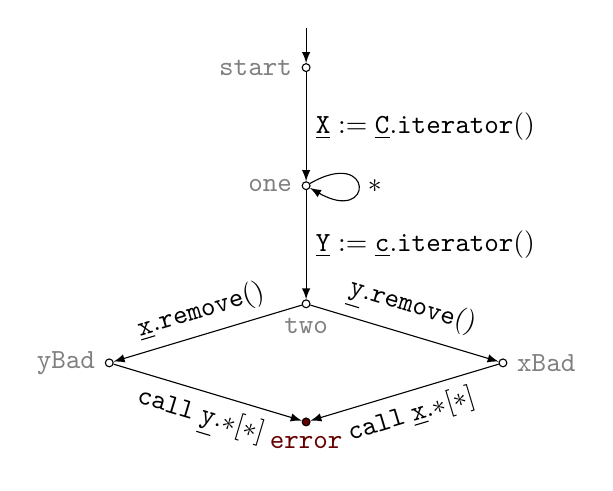
\begin{tikzpicture}
  \def\x{2.5}
  \def\y{1.5}
  \tikzset{vertex/.style={draw,circle,inner sep=1pt}}
  \tikzset{transition/.style={->,>=latex}}
  \tikzset{every label/.style={gray}}
  \node[vertex] (start) at (0,0) [label=left:\texttt{start}] {};
  \node[vertex] (one) at (0,-1*\y) [label=left:\texttt{one}] {};
  \node[vertex] (two) at (0,-2*\y) [label=below:\texttt{two}] {};
  \node[vertex] (xBad) at (1*\x,-2.5*\y) [label=right:\texttt{xBad}] {};
  \node[vertex] (yBad) at (-1*\x,-2.5*\y) [label=left:\texttt{yBad}] {};
  \node[vertex,fill=darkred] (error) at (0,-3*\y) [label=below:\textcolor{darkred}{\texttt{error}}] {};
  \draw[transition] (0,0.5)--(start);
  \draw[transition] (start)--node[right]{$\pattern X:=\pattern C.\mathtt{iterator}()$} (one);
  \draw[transition] (one) .. controls +(30:1cm) and +(-30:1cm) .. node[right]{$*$} (one);
  \draw[transition] (one)--node[right]{$\pattern Y:=\pattern c.\mathtt{iterator}()$} (two);
  \draw[transition] (two) -- node[sloped,above]{$\pattern y.\mathtt{remove}()$} (xBad);
  \draw[transition] (two)--node[sloped,above]{$\pattern x.\mathtt{remove}()$} (yBad);
  \draw[transition] (xBad)--node[sloped,below]{$\mathtt{call}\;\pattern x.{*}[*]$} (error);
  \draw[transition] (yBad)--node[sloped,below]{$\mathtt{call}\;\pattern y.{*}[*]$} (error);
\end{tikzpicture}
\\[2ex]
\begin{Verbatim}[commandchars=\\\{\}]
property InvalidateOtherIterators
  observe <java.util.\{Collection,Iterator\}.*>
  prefix <java.util.\{Collection,Iterator\}>
  start -> start: *
  start -> one:  \pattern{X} := \pattern{C}.iterator()
  one -> one:    *
  one -> two:    \pattern{Y} := \pattern{c}.iterator()
  two -> yBad:   \pattern{x}.remove()
  two -> xBad:   \pattern{y}.remove()
  yBad -> error: call \pattern{y}.*[*]
  xBad -> error: call \pattern{x}.*[*]
\end{Verbatim}
\caption{Property {\tt InvalidateOtherIterators} in diagram (above) and textual form (below).
}
\label{fig:first.topl}
\end{figure}
%
\begin{figure}[t]
{\def\s#1{\text{\Verb@#1@}}
 \def\m#1{\PY{n+na}{#1}}
 \def\t#1{\mathtt{#1}}
 \def\cmt#1{\textcolor{gray}{\text{// #1}}}
\begin{align*}
&\{\;(\start,[])\;\} \\
&\s{Iterator<Integer> i = c.\m{iterator}();}  \quad \cmt{\bf \it Step 1} \\
&\cmt{Assume {\tt c} holds $1$, and {\tt i} holds $2$ } \\
& \begin{aligned}
  \{\;&(\start,[]),\
      &(\t{one},[c:1,x:2])\;\}
  \end{aligned}\\
&\s{Iterator<Integer> j = c.\m{iterator}();}  \quad \cmt{\bf \it Step 2} \\
&\cmt{Assume {\tt j} holds $3$} \\
& \begin{aligned}
  \{\;&(\start,[]),\
      &(\t{one},[c:1,x:2]),\
      &(\t{one},[c:1,x:3]),\
   \end{aligned}\\
& \begin{aligned}   
      & \quad (\t{two},[c:1,x:2,y:3])\;\}
  \end{aligned}\\
&\s{i.\m{next}();} \quad \cmt{\bf \it Step 3} \\
& \begin{aligned}
  \{\;&(\start,[]),\
      &(\t{one},[c:1,x:2]),\
      &(\t{one},[c:1,x:3]),\
   \end{aligned}\\
& \begin{aligned}   
      & \quad (\t{two},[c:1,x:2,y:3])\;\}
  \end{aligned}\\
&\s{i.\m{remove}();} \quad \cmt{\bf \it Step 4}  \\
& \begin{aligned}
  \{\;&(\start,[]),\
      &(\t{one},[c:1,x:2]),\
      &(\t{one},[c:1,x:3]),\
   \end{aligned}\\
& \begin{aligned}   
      & \quad (\t{yBad},[c:1,x:2,y:3])\;\}
  \end{aligned}\\
&\s{j.\m{next}()} \quad \cmt{\bf \it Step 5}  \\
& \begin{aligned}
  \{\;&(\start,[]),\
      &(\t{one},[c:1,x:2]),\
      &(\t{one},[c:1,x:3]),\
   \end{aligned}\\
& \begin{aligned}   
      & \quad (\error,[c:1,x:2,y:3])\;\}
  \end{aligned}\\
\end{align*}}
\caption{Running trace of {\tt InvalidateOtherIterators}. Lines \{in curly brackets\} describe automaton's states;
lines in \texttt{monotype} show executing statements;
// are comments.}
\label{fig:first.steps}
\end{figure} % >>>
\autoref{fig:first.steps} shows an execution of the program in \autoref{fig:first.java} and an automaton for \texttt{InvalidateOtherIterators}.
At a given moment, the automaton has a set of active states.
A state is a pair of a vertex and a store.
The store is a memory that holds (automaton) variables.
Technically, it is a finite partial map from variables to values.
We write $[k_1:v_1,k_2:v_2]$ for the finite partial map that maps key~$k_1$ to value~$v_1$, and key~$k_2$ to value~$v_2$.
The empty map is denoted by~$[]$.

The automaton has variables $x$,~$y$, and~$c$.
At vertex \texttt{one} the variables $x$~and~$c$ are initialized;
at \texttt{two} the variables $x$,~$y$, and~$c$ are initialized.
At vertex \texttt{one} $x$~is an iterator for a collection~$c$, and
at \texttt{two}, $x$~and~$y$ are both two iterators for the same collection~$c$.
Notice that~\Verb@c@ is a program variable whereas~$c$ is an automaton variable.
The same name was chosen because the two variables always hold the same value in this example.
In general, however, program variables and automaton variables live in different name-spaces, and may hold different values.

To avoid confusion, program variables are typeset in \Verb@monotype@ (\Verb@c@,~\Verb@i@,~\Verb@j@).
Automaton variables are typeset in \textit{italics} ($c$,~$x$,~$y$) and do \emph{not} appear in the property.
Instead, automaton variable \emph{patterns} appear in the property, and they are typeset in \texttt{\underline{underlined monotype}} (\pattern c,~\pattern C, \pattern x, \pattern X, \pattern y,~\pattern Y).
The interaction between patterns and the automaton's memory is as follows: uppercase patterns write to the automaton memory, and lowercase patterns read from the automaton memory and act as a guard on the transition.

We now illustrate all this by going through the execution step by
step.

\paragraph{Step~1.}

Initially, only the state $(\start,[])$ is active.
The outgoing transition of vertex \start is labeled by $\pattern X:=\pattern{C}.\mathtt{iterator}()$ and the first executed statement is \verbline[.]{i = c.\PY{n+na}{iterator}()}
A method call matches a label when
\begin{itemize}
\item[(a)] the called method matches the method pattern, and
\item[(b)] the program values match their corresponding patterns.
\end{itemize}
By definition, any value matches an Uppercase pattern.
So here, the values of \Verb@i@~and~\Verb@c@ match the patterns \pattern X~and~\pattern C.
The method itself also matches the method pattern.
For simplicity, we ignore argument types and identify Java methods only by their fully qualified name and their arity.
The called method \texttt{iterator} is in the class \texttt{ArrayList} and has arity~$1$.
We identify it as follows.
\verbline{java.lang.ArrayList.iterator[1]}
The \texttt{prefix} directives, allows us to write the method pattern \Verb@iterator[1]@
and have it expanded to the following:
\begin{align*}
&\text{\Verb@java.util.Collection.iterator[1]@} \\
&\text{\Verb@java.util.Iterator.iterator[1]@}
\end{align*}
Similar to the \texttt{observe} directives, it means that these two methods \emph{and} all those that override them match.
Here, \texttt{ArrayList} implements \texttt{Collection} and so\\
\texttt{ArrayList.iterator} matches.

Thus, all conditions are met to enable the transition from \start to \texttt{one}.
When the transition is performed, the values that matched \pattern X~and~\pattern C are written in the automaton variables $x$~and~$c$.
For concreteness, let us assume these values are $1$~and~$2$. When the
program runs, these values will be the memory addresses of the objects
\Verb@c@ and \Verb@i@, so $1$ and $2$ are unlikely values, but for the
example they suffice.
After the transition is performed, the state $(\mathtt{one},[c:1,x:2])$ is active.
The state $(\start,[])$ remains active because the transition \verbline{start -> start: *} is also enabled and performed.

\paragraph{Step~2.}
For the second step, the statement to be executed is \verbline[.]{j = c.\PY{n+na}{iterator}()}
Now we need to consider, in turn, the two active states \[\{(\start,[])\quad\text{and}\quad(\texttt{one},[c:1,x:2])\}\]
For $(\start,[])$ the same reasoning as for step 1 holds, so the states $(\start,[])$ and $(\mathtt{one},[c:1,x:3])$ are active after step~2.
Note that now the automaton variable~$x$ remembers the value of the program variable~{\tt j}.
For $(\texttt{one},[c:1,x:2])$ we look at the outgoing transitions from vertex {\tt one}.
\begin{align*}
\text{\Verb@one -> one@} &: * \quad \mbox{ and } \quad \\
\text{\Verb@one -> two@} &: \text{\Verb@\pattern Y := \pattern c.iterator()@}
\end{align*}
The first transitions is always enabled, and performing it keeps states with vertex \texttt{one} active.
The second transitions has two patterns, \pattern Y~and~\pattern c.
The uppercase pattern~\pattern Y always matches, whereas
pattern \pattern c matches only the value held by the automaton variable~$c$.
In this case, $c$ was set in the previous step to the value of the program variable~\texttt{c}.
Therefore, the transition from~\Verb@one@ to~\Verb@two@ is performed and the state $(\mathtt{two},[c:1,x:2,y:3])$ is activated.

\paragraph{Step~3.}

The third step involves the statement
\[\text{\Verb+\PY{n}{i}\PY{o}{.}\PY{n+na}{next}\PY{o}{(}\PY{o}{)}\PY{o}{;}+}\]
which matches no label of outgoing transitions of the currently active vertices (that is, \start, {\tt one}, and {\tt  two}).
Therefore, although the program proceeds, the set of active states of the automaton remains unchanged.

\paragraph{Step~4.}

In the fourth step, the transition $\texttt{two}\to\texttt{yBad}$ is performed.
Notice that the pattern $\pattern{x}.\mathtt{remove}()$ does not have a left-hand side, which simply means that the returned value is irrelevant for this transition.
The states corresponding to vertices \start and {\tt one} remain unchanged, because their outgoing transitions are disabled.
However,  the outgoing transition of state {\tt two} is enabled, and therefore {\tt yBad} becomes active.

\paragraph{Step~5.}

For the fifth and final step, the statement to be executed is \verbline[.]{j.\PY{n+na}{next}()}
The label of the outgoing transition  \[\mathtt{call}\;\pattern{y}.{*}[*]\] of the active state $(\texttt{yBad},[c:1,x:2,y:3])$
has two distinguishing features: the~$*$ as a method name and the tag \texttt{call}.
As before, in order to match the method name, the prefixes
\Verb@java.util.Collection.*[*]@ as well as \Verb@java.util.Iterator.*[*]@
are prepended.
Then the $*$s are expanded, taking into account the \texttt{CLASSPATH}.
One expansion, \Verb@java.util.Iterator.next@, is indeed
overridden by the method that is actually called and therefore 
we have a match.

The tag {\tt call} is used when we want the automaton to take a transition precisely at call-time of a method invocation.
The automaton expresses that a call to one of {\tt j}'s methods while vertex \texttt{yBad} is active constitutes an error.
Notice that this is different from a label like $\pattern X:=\pattern C.\mathtt{iterator}()$ which may match only after the return value is known.

\medskip
The execution we stepped through reaches the \error vertex, so we conclude that the property is violated.
Notice that in order to find a counterexample we need to keep track of the relation between several objects, in particular that iterators {\tt i} and {\tt j} are for the same collection {\tt c}.

% >>>
\subsection{Heap Shape and Values Sensitive Properties}  % <<<
One interesting kind of properties for object-oriented programs is the ability to reason about the shape of the heap composed by the allocated objects.
The following TOPL properties test the shape of a linked list and
reports an error if it is cyclic or it has the pan-handle shape (i.e.,
there is a lasso at some point). Directives are omitted.
%
\delimitVerbatim
\begin{Verbatim}[commandchars=\\\{\}]
 property ListNotCyclic
   start -> start: *
   start -> a: \pattern{X} := *.getList()
   a -> a:     \pattern{X} := x.next()
   a -> b:     \pattern{Y} := x.next()
   b -> b:     \pattern{Y} := y.next()
   b -> error: x := y.next()
   a -> error: x := x.next()
\end{Verbatim}
\delimitVerbatim
The idea is that this property will bind the automaton variable $x$ with any possible object in the list, and the $y$ with any possible successors (via the next field) of the current binding of $x$.
Therefore, if there is a lasso, in the list, this will be detected when a new biding of $y$ via a \texttt{b -> b} becomes equal to the binding of $x$.
The transition \texttt{a ->error} detect the case where there is an object pointing to itself.


The following property detects when a dictionary overwrite one of its bindings.
\delimitVerbatim
\begin{Verbatim}[commandchars=\\\{\}]
 property BadDictionary
   message "dictionary overwrites its bindings"
   observe <Dictionary.*>
   prefix <Dictionary>
   start -> start: *
   start -> written:   \pattern{D}.put(\pattern{K}, \pattern{V})
   written -> written: d.put(k, \pattern{V})
   written -> error:   !v := d.get(k)
\end{Verbatim}
\delimitVerbatim
The overwrite is detected by the guard which checks if the value associated with a key $k$ is the same as the original binding recorded in the automaton variable $v$.

% >>>
\subsection{Taint Properties} % <<<

\rg{TODO: Explain how to express the generic taint property.}

% >>>
\subsection{Iterating Dirty Ropes} % <<<

\rg{TODO: Revisit the motivating example.
Ropes may represent strings.
So, ropes may be tainted or not.
Also, one could iterate over a subrope.}

% >>>
% >>>
\section{Implementation} \label{sec:implementation} % <<<

Our tool\footnote{\url{http://rgrig.github.com/topl}} checks whether a Java program violates a TOPL property.
The tool consists of two parts: a compiler and a checker.
The TOPL compiler ({\tt toplc}) instruments Java bytecode;
The TOPL checker (class {\tt topl.Checker}) monitors the execution and reports violations.
\autoref{architecture} depicts how the compiler and the checker fit together, thus summarizing our runtime checking technique.

\begin{figure*}[t]
\begin{center}
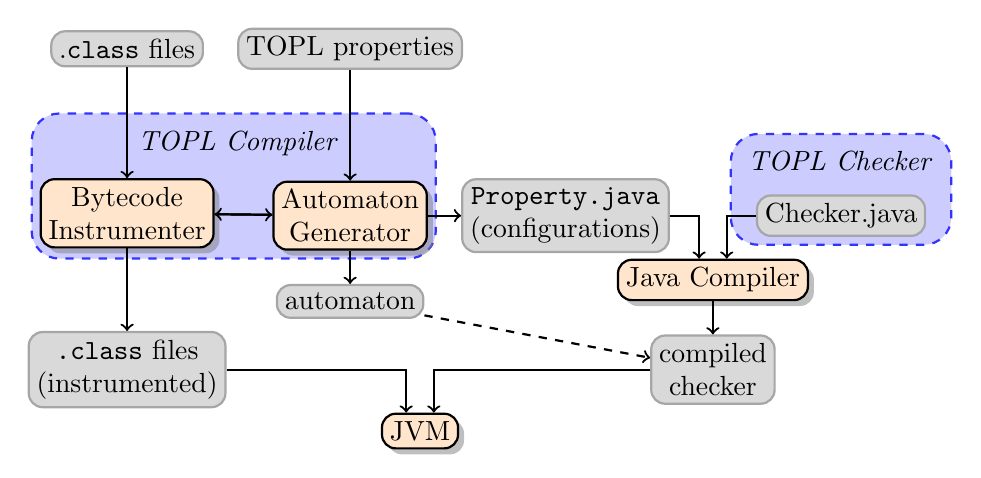
\begin{tikzpicture}[node distance=12pt, auto]
\tikzstyle{system}=[rectangle,
                                draw=blue!80,
                                fill=blue!20,
                                inner sep=0.1cm,
                                rounded corners=10pt,
                                style=dashed,thick]
\tikzstyle{program}=[rectangle,
                                  draw=black,
                                  fill=orange!20,
                                  inner sep=0.1cm,
                                  rounded corners=5pt,
                                  style=thick,
                                  drop shadow]
\tikzstyle{data}=[rectangle,
                            draw=gray!70,
                            fill=gray!30,
                            inner sep=0.1cm,
                            rounded corners=5pt,
                            style=thick]
\node[data] (classes) {{.\tt class} files};
\node[data, right=of classes] (properties) {TOPL properties};

\node[below=of classes] (classesd) {};
\node[below=of properties] (propertiesd) {};

\node[program, below=40pt of classes, align=center] (instrumenter)
  {Bytecode\\Instrumenter};
\node[program, below=40pt of properties, align=center] (genautomaton)
  {Automaton\\Generator};

\node[data, right=of genautomaton, align=center] (javaproperties)
  {{\tt Property.java}\\(configurations)};
\node[data, below=of genautomaton] (automaton) {automaton};
\node[right=of javaproperties] (javadummy) {};
\node[data, right=of javadummy] (checker) {Checker.java};
\node[program, below=of javadummy] (javac) {Java Compiler};

\node[data, below=of javac, align=center] (classproperties)
  {compiled\\checker};
\node[data, align=center] at (instrumenter |- classproperties)
  (instrclasses) {{\tt .class} files\\(instrumented)};
\node at ($(instrclasses)!.5!(classproperties)$) (classdummy) {};
\node[program, below=of classdummy] (jvm) {JVM};

\node[above=5pt] at ($(instrumenter.north)!.5!(genautomaton.north)$) (topllabel) {\emph{TOPL Compiler}};
\node[above=5pt of checker] (checkerlabel) {\emph{TOPL Checker}};
\begin{pgfonlayer}{background}
  \node[system, fit = (topllabel) (instrumenter) (genautomaton)] (TOPLC) {};
  \node[system, fit = (checker) (checkerlabel)] (CHECKER) {};
\end{pgfonlayer}

\path[thick, ->]
(classes) edge (instrumenter)

(genautomaton) edge (instrumenter)
(instrumenter) edge (genautomaton)

(properties) edge (genautomaton)
(genautomaton)  edge (javaproperties)
(javac) edge (classproperties)

(genautomaton) edge (automaton)

(instrumenter) edge (instrclasses);

\draw[thick, ->]
(instrclasses) -| ($(jvm.north)-(5pt,0)$);
\draw[thick, ->]
(classproperties) -| ($(jvm.north)+(5pt,0)$);
\draw[thick, ->]
(javaproperties)  -| ($(javac.north)-(5pt,0)$);
\draw[thick, ->]
(checker)  -| ($(javac.north)+(5pt,0)$);

\draw[thick, ->, dashed]
(automaton) -- (classproperties);
(\end{tikzpicture}

\caption{Architecture of the TOPL tool}
\label{architecture}
\end{center}
\end{figure*}

The compiler takes as input a Java project and a set of TOPL properties.
The Java project is defined to be all files in a given directory, recursively descending into jar files, zip files, and subdirectories.
The compiler produces (1)~a copy of the Java project with the class files instrumented, and (2)~a TOPL automaton.
The bytecode instrumentation and the construction of the TOPL automaton are intertwined.
On one hand, only the Java methods relevant to the given TOPL properties are instrumented.
On the other hand, the construction of the TOPL automaton relies on the inheritance tree of the Java project.
For example, suppose that a TOPL property mentions the method {\tt next} from the interface {\tt Iterator}.
Then, on one hand, all the methods that implement {\tt Iterator.next} are instrumented and, on the other hand, the corresponding guard in the automaton will match all these methods.

The compiler also performs two secondary tasks, for convenience.
First, it inserts a copy of the checker in the instrumented version of the Java project.
Second, it generates a Java file that activates and configures the checker.
It is this file that must be recompiled if one wishes to change the parameters of the checker, such as the maximum number of active states to track.
Because of these convenience features, all the user needs to do next is run the instrumented version of the Java project.

The checker logs property violations to {\tt System.err}.
The configuration parameters of the checker include:
\begin{itemize}
\item \emph{History length}---how many events to remember.
  A high value reports more events that led to \error.
  A low value reduces the space and time overhead.
\item \emph{Maximum number of active states}.
  A high value increases the chances of detecting violations.
  A low values reduces space and time overhead.
\item \emph{Collect call stacks}.
  A {\tt true} value includes call stacks in violation reports.
  A {\tt false} value reduces the space and time overhead.
\end{itemize}

\subsection{The TOPL Compiler} \label{sec:toplc} % <<<

The compiler has six phases, which are described below.

\paragraph{Parsing and Desugaring.}
TOPL properties are read first, before the Java project.
The parser desugars the TOPL properties into a simpler, intermediate form where
\begin{itemize}
\item Method-name patterns are prefixed according to the {\tt prefix} directive.
\item Lowercase patterns and constant patterns are turned into guards.
\item Uppercase patterns are turned into actions.
\item Transitions of length 2 or of length 1 are built according to whether the guards and the actions refer to both call-time and return-time or not. (In particular, there are no transitions of length~$0$.)
\end{itemize}
The parser builds an AST that closely follows the language for which we gave formal operational semantics.

\paragraph{Static Checks.}
Next, the compiler checks that the property is well-formed:
\begin{itemize}
\item two parallel writes to automaton variables have distinct destinations;
\item reads from automaton variables must be preceded by writes.
\end{itemize}

The compiler warns if some vertices are unused.
Properties with unused vertices are still well-formed.
We plan to also statically check whether the automaton can never fail.

\paragraph{Generate Event Identifiers.}

In this phase, each observable method is assigned two identifiers, one for the call event and one for the return event.
A method is \emph{observable} when its full name or the full name of a method it overrides matches the {\tt observe} directive.
The bytecode is read to collect all method names and to build the inheritance tree.

\paragraph{Construct the Automaton.}

In this phase, all properties are merged into one automaton.
From now on vertices are integers, rather than strings.
All vertices that had the name \start are now in the set of start vertices;
all vertices that had the name \error now have an error message attached.
Each TOPL property has its own {\tt observe} directive.
This information must be encoded in the automaton:
Each vertex is given a set of event identifiers.

The guards of the automaton are of two kinds.
Those that test program values are essentially left unchanged in this phase.
Those that check the event type, the method name, and the method arity are all transformed into one guard that is represented by a set of event identifiers.
The evaluation of the guard at runtime is a set containment test.

The automaton is dumped into the file {\tt Property.text}.
The TOPL compiler does not interpret Java expressions.
If a guard compares a program value with a literal, then the literal is saved in an array in {\tt Property.java}, and {\tt Property.text} points to it.

\paragraph{Generate Checker Configurations.}

In this phase, which is intertwined with the previous one, the compiler generates a file {\tt Property.java}.
This file serves three purposes:
\begin{itemize}
\item
It contains an array with all the constants used in the TOPL property.
For example, if a guard requires that a certain argument equals the expression~$21/7$, then $21/7$ is stored in this array.
\item
It activates the checker.
The checker is inactive by default so that the Java standard library may be instrumented.
The JVM uses certain parts of the standard library during its own startup.
If those parts happen to be instrumented then they call into the checker.
If the checker is inactive it immediately returns and the execution continues.
If the checker would be active then it will call back into the standard library and the JVM will crash.
\item
For convenience, it contains code that configures the checker.
To change the parameters of the checker the user changes this code and recompiles {\tt Property.java}.
\end{itemize}

\paragraph{Instrumentation.}

In this phase, the bytecode of observable methods is instrumented.
The first and last actions performed by the instrumented version are calls to the method {\tt check} of the checker.
This method takes an event as an argument.
Each event carries an identifier and an array of {\tt Object}.
The array holds either the arguments, or the return value.

To instrument Java bytecode we use a fork of the library Barista~\cite{barista}.
The high-level bytecode representation of the original library is rather low-level.
For example, it still represents jumps as byte counts.
We changed Barista's high-level representation to make it easy to use for instrumentation.
Hence, we had to rewrite the code that transformed between the low-level and the high-level representation.
These changes amount to more than half our implementation effort.
(For example, adding the number of lines changed by each commit gives $48\rm\,K$.)

% >>>
\subsection{The TOPL Checker} % <<<

The checker logs the property violations that it detects.
Its components are:
\begin{itemize}
\item the data structures used to represent the automaton, and a parser that instantiates them while processing {\tt Property.text};
\item the data structures used to represent the current state of the checker;
\item the code that handles one incoming event;
\item the code that garbage collects old states; and
\item the code that chooses which of the active states to forget.
\end{itemize}

\paragraph{States.}
The checker maintains a set of active states.
A state consists of vertex, a store, and a queue of events yet to be processed.
The vertex is simply an integer.
The store maps automaton variables ({\tt in}) to values ({\tt Object}).
A maximum size of~$2$ for the queue of events suffices because transitions have depth $1$~or~$2$.
(If all transitions would have the same depth, then one global queue of events would suffice.
Since the transition depth is bounded the checker could still use a couple of global queues, but we chose for now an implementation that is easy to generalize.)

States are created produced by applying an action to another state (called the parent).
For error reporting, each state keeps track of its parent.
An active state with $\ge2$~outgoing transitions produces $\ge2$~active states for the next time step.
The new active states and their parent are likely to have similar stores.
The implementation takes advantage of this fact by using persistent (functional) sets for bindings to represent stores; more precisely, we use treaps~\cite{DBLP:conf/focs/AragonS89}.

\paragraph{Step.}

The procedure from \autoref{fig:checker.step} builds the set~$A$ of states that are active after processing one event.
It corresponds to the operational semantics (\autoref{def:rcg}), but is written in an imperative style.
For each transition outgoing from a vertex, lines~\hbox{11--17} follow the step transitions from \autoref{def:rcg}.
Line~17 is reached if the rule (Step) does not apply, and execution continues with the next outgoing transition.
Line~18 is reached if the rule (Step) does apply.
Its effect is recorded by adding a new state to set~$A$
If rule (Step) did not apply for any outgoing transition, then rule (Silent) is applied by lines~22--23.

\begin{figure*}[t]
\begin{center}
\begin{alg}
\^  $\proc{Step}(e)$
\=  $A := \emptyset$
\=  for each active state $s$
\+    if $\mathit{vertex}(s)$ does not observe $\mathit{id}(e)$
\+      insert $s$ into $A$
\=      continue from $3$
\-    push $e$ to the queue $\mathit{events}(s)$
\=    if $\mathit{events}(s)$ is shorter than the longest transition from $\mathit{vertex}(s)$
\+      continue from $3$
\1    $\mathit{skip}:=\mathsf{true}$
\=    for each transition $t$ outgoing from $\mathit{vertex}(s)$
\+      $\sigma := \mathit{store}(s)$,\quad $E := \mathit{events}(s)$
\=      for each step $\tau$ of $t$
\+        pop $\varepsilon$ from the queue $E$
\+        if $\proc{Guard}(\tau, \varepsilon, \sigma)$
\+          $\sigma := \proc{Action}(\tau, \varepsilon, \sigma)$
\-        else
\+          continue from 11
\2      $\mathit{skip}:=\mathsf{false}$
\=      insert state $(\mathit{target}(t), \sigma, E)$ into $A$
\=      if $\mathit{target}(t)$ is an error vertex, report the error
\=      if \textit{skip}
\+        $s' := s$
\=        insert state $s'$ with one event popped into $A$
\end{alg}
\bigskip
\caption{
  Executing one step.
  The code builds the set~$A$ of states that are active after processing one event.
}
\label{fig:checker.step}
\end{center}
\end{figure*}

\paragraph{Garbage Collection.}

States point to their parent when they are created.
But, if they continue to do so forever, then the memory footprint of the states would be proportional to the number of events received by the checker.
The space overhead would be too big for long running programs.
Usually, most of the states are not needed.
The typical property has a $*$-loop on the \start vertex.
An error trace going all the way back to the beginning would mention that this loop is taken many times before something interesting happens.
In general it is very unlikely that the user needs a trace with more than about $10$~states.
The history length~$h$ is one of the parameters configurable from {\tt Property.java}.

We should allow the Java~VM to garbage collect states that are not reachable in $h$~steps from some active state.
After each {\sc Step} we could do a BFS traversal with $h$~steps and set to {\tt null} the parent pointer of fringe states.
However, if there are $n$~active states, the traversal would take $O(nh)$~time.
The procedure {\sc Step} takes $O(nd)$~time, where $d$ is the maximum out-degree of the property.
So, the checker would become much slower if $h>d$, which usually is the case.

One solution could be to perform the BFS once in every $h/d$~steps.
The solution we implemented tries to better address the average case.
We remember the number~$m$ of states seen by a BFS, and perform the next BFS after $\sim m$~new states were created.

\paragraph{Approximation.}

\autoref{fig:completeness} illustrates why the checker needs unbounded memory if it must not miss bugs exhibited by an execution.
The problem is essentially that the set of active states of a nondeterministic automaton is unbounded.
Of course, an arbitrary amount of space overhead is unacceptable.

\begin{figure}[t]
\begin{center}
\begin{Verbatim}[commandchars=\\\{\}]
\PY{k+kn}{import} \PY{n+nn}{java.util.*}\PY{o}{;}
\PY{k+kd}{public} \PY{k+kd}{class} \PY{n+nc}{Completeness} \PY{o}{\PYZob{}}
   \PY{n}{Collection} \PY{n}{c}\PY{o}{;}
   \PY{n}{Random} \PY{n}{r}\PY{o}{=}\PY{k}{new} \PY{n}{Random}\PY{o}{(}\PY{o}{)}\PY{o}{;}
   \PY{k+kd}{public} \PY{k+kt}{void} \PY{n+nf}{NeedsUnboundMemory}\PY{o}{(}\PY{k+kt}{int} \PY{n}{n}\PY{o}{)} \PY{o}{\PYZob{}}
      \PY{n}{Iterator}\PY{o}{[}\PY{o}{]} \PY{n}{a} \PY{o}{=} \PY{k}{new} \PY{n}{Iterator}\PY{o}{[}\PY{n}{n}\PY{o}{]}\PY{o}{;}
      \PY{k}{for} \PY{o}{(}\PY{k+kt}{int} \PY{n}{i}\PY{o}{=}\PY{l+m+mi}{0}\PY{o}{;} \PY{n}{i}\PY{o}{<}\PY{n}{n}\PY{o}{;} \PY{n}{i}\PY{o}{+}\PY{o}{+}\PY{o}{)} \PY{o}{\PYZob{}}
          \PY{n}{a}\PY{o}{[}\PY{n}{i}\PY{o}{]}\PY{o}{=}\PY{n}{c}\PY{o}{.}\PY{n+na}{iterator}\PY{o}{(}\PY{o}{)}\PY{o}{;}
          \PY{k}{if} \PY{o}{(}\PY{n}{r}\PY{o}{.}\PY{n+na}{nextBoolean}\PY{o}{(}\PY{o}{)}\PY{o}{)} 
	    \PY{k}{while} \PY{o}{(}\PY{n}{a}\PY{o}{[}\PY{n}{i}\PY{o}{]}\PY{o}{.}\PY{n+na}{hasNext}\PY{o}{(}\PY{o}{)}\PY{o}{)} \PY{n}{a}\PY{o}{[}\PY{n}{i}\PY{o}{]}\PY{o}{.}\PY{n+na}{next}\PY{o}{(}\PY{o}{)}\PY{o}{;}	
      \PY{o}{\PYZcb{}}\PY{o}{;}
      \PY{n}{a}\PY{o}{[}\PY{n}{r}\PY{o}{.}\PY{n+na}{nextInt}\PY{o}{(}\PY{n}{n}\PY{o}{)}\PY{o}{]}\PY{o}{.}\PY{n+na}{next}\PY{o}{(}\PY{o}{)}\PY{o}{;}
  \PY{o}{\PYZcb{}}\PY{o}{;}
\PY{o}{\PYZcb{}}
\end{Verbatim}

\caption{Counterexample to runtime completeness.}
\label{fig:completeness}
\end{center}
\end{figure}

Like in the case of trace lengths, we impose a limit that is fixed but configurable by the user.
In this case, however, we must also pick which active states to forget.
We implemented three strategies: random, newest, and oldest.
The words newest\slash oldest refer to a time that is attached to states, and is one more than the time of the parent state.
The time of a state is the number of times the (Step) transition of the operational semantics was taken in order to produce the state.

%\dinocomment{discuss about: conservative and transparent properties of an inliner}
%\dinocomment{talk about our strategy}

% >>>
% >>>
\section{Experimental Results}\label{sec:results} % <<<

Our interest in temporal properties of object-oriented programs was initially purely theoretical.
But we implemented our technique to ensure we are not dismissing an important issue as merely engineering.
In particular, without an implementation it is hard to judge if the performance penalty is acceptable.

\subsection{Methodology} % <<<

We expect our technique to be most useful during development.
Library writers will document temporal constraints in TOPL, not just in English.
Each library will have a testing version, obtained by instrumenting the bytecode with the TOPL properties.
Users will use the testing version of the library to ensure they use it correctly.
By the time end-users see the application, most temporal bugs are gone.
Back in the real world, we too would like to know if such a scenario is likely.
Alas, observing the effect of using TOPL during the life-time of a real project is rather time consuming.
We have to settle for less.

We measure the overhead on the test suite DaCapo~\cite{dblp:conf/oopsla/dacapo}, version~9.12.
DaCapo is a collection of automated tests that exercise large portions of code from open-source projects.
We focus on $3$~projects that are still widely developed and used: Tomcat, H2, and PMD\null.
These are all mature projects with many users.
DaCapo itself was used for many experiments by the research community.
Hence, we do not expect to find any bugs, but aim to measure the overhead.
For each project we write a few TOPL properties that encode information that exists in the code comments.
In fact, we identify these properties by searching the code for words with temporal connotations, such as `before' and `after'.

We measure both the time overhead and the space overhead.
The time overhead is reported measured for various configurations of the checker, and also for the original bytecode, with no instrumentation whatsoever.

All experiments are performed on the same machine.
The operating system kernel is Linux~2.6.32.
The Java VM has version~1.6.0\_20.
The processor is Intel i5 with $4$~cores at $3.33\rm\,GHz$.
The total system memory is $4\rm\,GiB$.

% >>>
\subsection{A Bug's Death} % <<<

The interface \texttt{ServletResponse} from Tomcat contains methods \texttt{getWriter} and \texttt{getOutputStream}.
The documentation of \texttt{getWriter} states that ``either this method or \texttt{getOutputStream} may be called to write the body, not both''.
We initially interpreted this comment as follows.
\eqquote{It is illegal to call both the method {\tt getWriter} and the method {\tt getOutputStream} on the same instance of {\tt ServletResponse}.}{eq:prop-ws-strong}
The TOPL checker reported many violations of~\eqref{eq:prop-ws-strong}.
We were not too surprised because we were unsure of the intended meaning of the comment.
We were surprised, however, that sometimes a {\tt null} dereference occurred in DaCapo itself.
We investigated.
The statement that threw a {\tt null}-pointer exception was the following:
\begin{align}\label{eq:npe-src}
\text{\Verb@if (log != null) log.write(b);@}
\end{align}
It must be that a concurrent thread sets {\tt log} to~{\tt null}.
The statement is located in the method {\tt write} of the class {\tt TeeOutputStream}.
The only method that sets {\tt log} to~{\tt null} is {\tt closeLog}, from the same class.
So, we wrote a TOPL property saying that \textit{executions of {\tt write} and {\tt closeLog} must not overlap in time}, and we asked for error reports that include call stacks.
Indeed, DaCapo's main loop sometimes calls {\tt closeLog} while the Tomcat server is printing.
%XXX\rg{Put here a trace for the error.}

TOPL helped us find a concurrency bug in the infrastructure of DaCapo.
First, the bytecode instrumented by TOPL helped us notice the problem.
The reason is \emph{not} that a certain interleaving became more likely.
Bug~2934521 of DaCapo mentions that exceptions of the Tomcat benchmark are silently ignored.
This is why the {\tt null}-dereference was not noticed before.
The TOPL checker tried to report an unrelated issue to {\tt System.err}.
DaCapo had redirected the standard error stream to its own class, which faulted.
TOPL caught the error and reported it as an internal issue, because no exceptions should be thrown while running the TOPL checker.
This is why we noticed the {\tt null}-dereference.
Second, TOPL helped us identify the data race.
It was easy to notice that statement~\eqref{eq:npe-src} should be atomic.
However, it would have been more difficult to figure out which threads exactly used the stream simultaneously.

We then tried a weaker version of property~\eqref{eq:prop-ws-strong}:
\eqquote{The stream and the writer of a response cannot both be used.}
{eq:prop-ws-weak}
This property involves three related objects.
The full TOPL property appears in~\autoref{fig:tomcat-prop}.
It turns out this property is also violated.
After reading the code to which the error traces pointed at, we noticed that the comments of some implementing classes weaken the contract:
They say that the stream and the response cannot be used without an intervening {\tt reset}.
In this case the comments on the interface {\tt ServletResponse} are arguably wrong, rather than the code.
This brings out another advantage of TOPL:
Since TOPL properties are processed by tools, they are less likely to become out-of-sync with the code.

% >>>
\subsection{Benchmarks} % <<<

\rg{TODO: Add the JDK properties from JavaMOP people.}
\rg{TODO: Clearly explain that our active configurations (not states, BTW) are \emph{not} the same at all with the number of monitors reported by the other runtime verification people.}

All three benchmarks are large open-source projects with many users and active developers.
The versions were current in 2009 when DaCapo-9.12 was released.

\paragraph{Tomcat 6.0.20.}
Tomcat is a servlet server; so, highly concurrent.
Servlets are Java programs that run in a webserver, extract data from {\tt ServletRequest}s , and send data into {\tt ServletResponse}s.
A response has two associated incoming channels: a stream and a writer.
The stream and the writer should not both be used.
Property~\eqref{eq:prop-ws-strong} is a strong interpretation of this constraint;
property~\eqref{eq:prop-ws-weak} is a weak interpretation of this constraint.
A response could be forwarded once the servlet sent data to it.
But, the servlet must commit a response before forwarding it, by calling {\tt fulsh} on the stream, on ther writer, or on the response itself.
This is the other property we checked.

\paragraph{H2 1.2.121.}
H2 is a database server.
We checked four properties for it.
Three properties express constraints on the order in which the methods of an interface may be called.
For example, a client should not attempt to ask for a row from a cursor that did not advance;
that is, for the interface {\tt Cursor}, the method {\tt next} must be called before calling method {\tt getSearchRow}.
The fourth property describes the contract of the class {\tt SysConstants}.
This class reads environment variables when it is loaded.
Its comments say that it is legal for a program to set these environment variables using the method {\tt System.setProperty}, provided that this is done before the Java VM loads the class {\tt SysConstants}.
It is easy to specify this property because TOPL intentionally treats the special methods {\tt <init>} and {\tt <clinit>} as if they are normal methods.

\paragraph{PMD 4.2.5.}
PMD looks for bugs, dead code, and a few other problems in Java code.
We checked five properties for it.
One of the five involves two objects:
A scope should be asked what is the definition of a name only if it already replied that it knows the name.

% >>>
\subsection{Overhead} % <<<

Instrumenting DaCapo, which has $160\rm\,MiB$, takes $7$~minutes.
One needs to instrument once for a given set of properties, because instrumentation is property-directed.
A change of a runtime parameter, such as the maximum number of tracked active states, requires recompiling the TOPL checker, but does not require re-instrumenting.

\paragraph{Space.}
Estimates of heap size showed no significant increase in memory use.
We used a simple method.
The heap of a Java program has three parts: used, garbage, and free.
The class {\tt Runtime} from the package {\tt java.lang} provides an estimate of the total size and of the free size.
The difference is an estimate of the used size, provided the garbage was collected immediately before.
We put this code, which estimates memory use, in the TOPL checker.
So, strictly speaking we did not estimate the memory use without the checker.
However, we used as a baseline a run that tracked no active state.
We also run the estimate for various other counts of tracked active states.

\paragraph{Time.}
\autoref{table:overhead} summarizes the experimental results.
The reference column shows the running time without any instrumentation.
A timeout signifies a time greater than the reference time~$\times100$.
All reported times are averaged over $10$~runs, and are accompanied by the unbiased estimate of standard deviation.
The TOPL checker essentially simulates a nondeterministic register automaton.
In theory the set of active states is unbounded, but we impose a size limit on it.
The table reports the running times for the instrumented bytecode when the size limit is $0$, $10^1$, $10^2$, $10^3$, and~$10^4$.

For tomcat the running time is essentially the same when tracking $\le10^4$ active states as it is when tracking $\le10^3$ active states.
This indicates that $\le10^3$ active states already exhaustively check the given properties.
For h2 the running time is more than $\times1.4$ the reference time even when the TOPL checker is not tracking any active state.
This indicates that we instrumented a simple method that runs often.

\begin{table*}[t]\centering
\begin{tabular}{@{}rr@{}lr@{}lr@{}lr@{}lr@{}lr@{}l}
  &&
  & \multicolumn{10}{c}{Number of tracked active states} \\ \cmidrule{4-13}
& \multicolumn{2}{c}{reference}
  &\multicolumn{2}{c}{$\le0$}
  &\multicolumn{2}{c}{$\le10^1$}
  &\multicolumn{2}{c}{$\le10^2$}
  &\multicolumn{2}{c}{$\le10^3$}
  &\multicolumn{2}{c}{$\le10^4$} \\ \midrule
tomcat
  & $5.3$ & $\pm0.1$
  & $5.4$ & $\pm0.1$
  & $5.6$ & $\pm0.2$
  & $9.0$ & $\pm0.3$
  & $43.5$ & $\pm1.2$
  & $43.9$ & $\pm1.0$ \\
pmd
  & $5.2$ & $\pm0.4$
  & $5.4$ & $\pm0.2$
  & $12.2$ & $\pm0.3$
  & $47.7$ & $\pm10.7$
  & \multicolumn{2}{c}{timeout}
  & \multicolumn{2}{c}{timeout}
  \\
h2
  & $6.6$ & $\pm0.2$
  & $9.5$ & $\pm0.2$
  & $130.1$ & $\pm12.2$
  & \multicolumn{2}{c}{timeout}
  & \multicolumn{2}{c}{timeout}
  & \multicolumn{2}{c}{timeout}
  \\
\end{tabular}
\caption{
  Experimental Results.
  Times are in seconds, averaged over $10$~runs.
}\label{table:overhead}
\end{table*}

% >>>
% >>>
\section{Related Work}\label{sec:related} %<<<

TOPL is an application of automata theory to program verification.
Consequently, there is related work in the area of automata theory and there is related work in the area of program verification.

TOPL automata are a variant of {\it register automata\/}~\cite{dblp:conf/focs/kaminskif90}, which were introduced in~1990.
Register automata work with infinite alphabets, as do a few other types of automata~\cite{dblp:conf/csl/segoufin06}.
Intuitively, such models are a good fit for expressing properties of programs because the set of program values is infinite.
For example objects could be instantiated inside non-terminating loops.
Our paper exhibits a working runtime verification system based on register automata, thus validating the intuition.

\rg{Add a section that imports results from RAs, and then summarize here:
closure under various operations, projection on~$C^*, $emptiness, language inclusion, universality, nondeterminism.}
\rg{TODO: Discuss rollback, once it's settled in the body of the article.}
\rg{TODO: In future work, discuss other RA news that may be relevant.}

Related work from the area of program verification splits by programming paradigm (object-oriented or functional) and by time of checking (runtime or static).
The work on runtime verification of object-oriented programs is closest to TOPL\null.

{\it JavaMOP\/}~\cite{dblp:journals/sttt/meredithjgcr12} and {\it tracematches\/}~\cite{dblp:conf/oopsla/allanachklmsst05} are the main runtime verification systems that handle multiple objects.
They differ in many details, but the essential ideas fit a common intuition.
To communicate this intuition we depart from the terminologies of \cite{dblp:journals/sttt/meredithjgcr12}~and~\cite{dblp:conf/oopsla/allanachklmsst05}, which are themselves different from each other.
The alphabet is~$\Sigma=C\times V$, where $C$~is a finite set of constants and $V$~is an infinite set of values.
The task is to build a recognizer $\Sigma^*\to\B$.
Both approaches build upon a basic recognizer $C^*\to\B$ over finite alphabets.
Tracematches specify this recognizer by regular expressions, while JavaMOP supports several other logics.
Both approaches make further assumptions on the structure of~$V$, and then define a way to specify a family $P\subset\Sigma\to\B$ of predicates over letters.
Each such predicate~$p\in P$ determines a slice $\tau_p\in C^*$ of the trace $\tau\in\Sigma^*$ by retaining exactly those constants from letters satisfying~$p$.
The trace~$\tau$ is recognized when any of its slices satisfy the basic recognizer.

The implementation of JavaMOP is more efficient than that of tracematches~\cite{dblp:journals/corr/abs-1112-5761}.
\rg{TODO: Comment on the efficiency of JavaMOP compared to TOPL after I do the experiments.}

There exist properties expressible in TOPL that cannot be expressed as JavaMOP properties or as tracematches.
Consider the language of traces
${\rm s}(v_1) {\rm d}(v_1,v_2){\rm d}(v_2,v_3)\ldots{\rm d}(v_{n-1},v_n){\rm t}(v_n)$
with $v_i=v_j$ if and only if $i=1$ and $j=n$.
This is a taint property: the dirty value~$v_1$ is produced, then comes a chain in which new dirty values are derived from old dirty values, and finally the dirty value~$v_n$ is misused.
It cannot be recognized in the framework used by JavaMOP and by tracemaches because slicing is pointwise.
\rg{Add this property as an example and then just refer to its name.}
\rg{TODO: Email Grigore Rosu to make sure this is true.}
\rg{TODO: Add the Singleton pattern as another example of what they can't handle, because they do not have negation.}

Any algorithm that analyzes or transforms JavaMOP properties must be specific to a certain plugin because the formalization of the framework~\cite{dblp:journals/corr/abs-1112-5761} imposes no constraint on recognizers $C^*\to\B$.
In contrast, any algorithmic result discovered for register automata implies one for TOPL properties.
For example we know that the emptiness problem is decidable, and we know that it is impossible to compute the negation of a property.

{\it Tracematches\/}~\cite{dblp:conf/oopsla/allanachklmsst05} are likely to have the exact same expressivity as JavaMOP with the plugin for regular expressions.
But, we are unaware of a fully formal comparison.
Tracematches evolved from the work on aspect-oriented programming.
Unsurprisingly, the user may specify arbitrary code to run when a match is found.
The formal semantics ignore this arbitrary code and how it could influence further matches.


TOPL takes inspiration from several existing  languages for type-state~\cite{strom1986,dblp:conf/oopsla/bierhoffa07,dblp:conf/oopsla/naeeml08,disney2011,ball2002}, but  it allows articulating  relationships and interactions among several objects.
Existing techniques for type-state aim at decomposing properties involving several objects into specifications reflecting the point of view of {\em one} single object.
TOPL, in contrast,  intentionally avoids such decomposition.
Parkinson~\cite{parkinson-iwaco2007} argues that invariants involving several objects are often better than one-object invariants.
Similarly, we believe that temporal properties that naturally involve a plurality of objects are easier to express and reason about if they are \emph{not} decomposed.
One language in the literature sharing this point of view is tracematches~\cite{dblp:conf/oopsla/allanachklmsst05}.
The ability of TOPL automata to store,  update, and compare values of their (infinite alphabet) registers combined with nondeterminism makes TOPL strictly more expressive than tracematches.

Our work 
extends the fundamental concept 
of typestate~\cite{strom1986} originally developed for imperative programs
by integrating notions typical of object-oriented programs.
 We are certainly not the first in doing this: there are several extensions of typestate to object-oriented programming in the literature.
A modular static verification method for typestate protocols is introduced in~\cite{dblp:conf/oopsla/bierhoffa07}.
The specification method is based on linear logic and relations among objects in the protocol are monitored by a tailored system of permissions.
The method is highly modular and presumably efficient.
The specification of the interactions among objects by means of permissions adds an extra level of machinery which increases the gap between the intuitive protocol description and its formalization.
Similarly~\cite{deline2004,dblp:conf/sigsoft/BierhoffA05} provide a mean to specify typestate properties that belong to a single object.
The specified properties are reminiscent of contracts or pre/post-conditions for methods and can deal with inheritance.
In~\cite{dblp:conf/issta/FinkYDRG06} the authors present sound verification techniques for typestate properties of Java  programs.
Their approach is divided in several stages with different verifiers varying for cost and precision.
In the early stages efficient but imprecise analyses are employed whereas more expensive and precise techniques are then progressively employed in later stages.
Every stage focuses on verifying only the parts of the code that previous stages failed to verify.
It is likely that  TOPL could be fruitfully combined with their analysis technique.

QVM~\cite{arnold:2008} is a runtime monitoring system tracking a subset of objects, chosen by
sampling. To ensure that the timing overhead of the monitoring is below a given target, the sampling rate is 
automatically adapted on the fly. For TOPL the control of the overhead is done manually by  the programmer who can tune the quantity of info to be tracked.
To improve performance,  the implementation of the QVM monitor is in the virtual machine,which, as a consequence makes it less portable for
different virtual machines. 
%\dd{how do we defend ourselves for the fact that we cannot predict
%  overhead?}\rlp{by experiments?}
An automata-based formalism for specifying properties of software interfaces was introduced in~\cite{dblp:conf/sigsoft/AlfaroH01} .
This language aims at capturing assumptions about the order in which the methods of a component are called and the order in which the component calls external methods.
In contrast to TOPL, this formalism is mainly used to check the compatibility of the interfaces of two components and it is designed to be applied at  model level rather than code level.
A specification language for interface checking aimed at C programs (called SLIC) is introduced in~\cite{ball2002}.
Differences between SLIC and TOPL include: the use (in SLIC) of non-determinism to encode universal quantification of dynamically allocated data, and the  ability to have complex code in the automaton transitions.
TOPL specifications naturally express universally quantified properties over data structures and for computability reasons,  we have chosen to limit the  actions performed during automaton transitions.
Simple SLIC specifications are verified by  the SLAM verifier~\cite{dblp:conf/cav/ballr01}.
While SLAM specialises on device drivers and checks client conformance rather than full protocols,
very general specifications of object-oriented program behaviour can be given in JML~\cite{jml} and Spec$\sharp$~\cite{DBLP:journals/jot/BarnettDFLS04}. However the latter two languages focus on class specifications and do not have temporal features.

In~\cite{disney2011} contracts are used to express legal traces of programs in a functional language with references.
The contracts specify traces as regular expressions over calls and returns, and hence, they resemble our automata, in a quite different setting.
Here, the specifications are function-centered, though, and again, capturing inter-object relations seems somewhat tricky.

ConSpec~\cite{DBLP:journals/entcs/AktugN08} is a language used to describe security policies.
Because ConSpec automatons are deterministic and have only a countable number of states, they cannot in principle express the property \texttt{InvalidateOtherIterators} (\autoref{sec:examples.steps}).


%\rg{I think the paper~\cite{dblp:journals/tocl/demril09} adds an operator to LTL to make it more expressive than register automata.
%We should discuss here, but I moved the citation out of the introduction.}
%\dinocomment{Add more on dynamic checks and byte code instrumentation}
%\dd{cite grigore rosu's work}
% >>>
\section{Conclusions and Future Work}\label{sec:conclusions} %<<<

\paragraph{Conclusions.}
We introduced TOPL---a language for expressing temporal safety properties for object-oriented programs via an extension of register automata.
TOPL can express constraints involving the relation of many objects at the same time.
Furthermore, we introduced a technique for checking at runtime the violation of the properties on Java program.
We have applied our technique to a variety of programs including large open source Java projects.
%
\paragraph{Future work.}
In the future, we intend to combine TOPL with  separation logic~\cite{reynolds2002} in order to deal with the heavy use of the heap and aliasing in object-oriented software.
Moreover, we aim at developing static analysis techniques for TOPL properties using the jStar framework~\cite{DBLP:conf/oopsla/DistefanoP08}.
This will require investigating suitable abstraction for obtaining meaningful and precise over-approximations of the state space of the programs.
Finally, we intend to develop a tailored bi-abduction inference technology~\cite{dblp:conf/popl/CalcagnoDOY09} which would help with scalability of the analysis.
\rlp{What about abstraction even for dynamic analysis?}
%>>>
\bibliographystyle{plain} % and appendix <<<
\bibliography{safety}

\appendix
\section{TOPL Syntax}
\label{app:syntax}
\begin{tabular}{l}
\grammar{
  Property& \b{property} Identifier Item\* \cr
  Item& Prefix \| Observe \| Transition \cr
  Prefix& \b{prefix} \b< StringPattern \b> \cr
  Observe& \b{observe} \b< StringPattern \b> \cr
  Transition& Arc \b: Label \(\b, Label\)\* \cr
  StringPattern& \(Letter \| \b. \| \b* \| \b{\{} \| \b{\}} \| \b, \)\+ \cr
  Arc& Vertex \b{->} Vertex \cr
  Label& Tag\? MethodPattern \cr
  Vertex& Identifier \cr
  Tag& \b{call} \| \b{return} \cr
  MethodPattern& ResultPattern\? NamePattern ArgumentsPattern \cr
  ResultPattern& ValuePattern \b{:=} \cr
  NamePattern& StringPattern \cr
  ArgumentsPattern& \b( \(ValuePattern \(\b, ValuePattern\)\*\)\? \b) \cr
  ArgumentsPattern& \b[ IntegerPattern \b] \cr
  ValuePattern& \b* \| \b< Literal \b> \| UppercaseId \| LowercaseId \cr
  IntegerPattern& \b* \| IntegerLiteral \cr
}
\end{tabular}


\begin{figure*}[h]\label{fig:tomcat-prop}
\begin{Verbatim}
property InterleavedResponse2
  // vertex names: w = got writer; W = used writer; similarly for s, S
  message "Incompatible methods for putting data into a response were used."
  observe <javax.servlet.ServletOutputStream.*>
  observe <java.io.PrintWriter.*>
  observe <javax.servlet.ServletResponse.{getOutputStream,getWriter}>
  prefix <javax.servlet.ServletResponse>
  start -> start: *
  start -> w: W := R.getWriter()
  start -> s: S := R.getOutputStream()
  w -> sw: S := r.getOutputStream()
  s -> sw: W := r.getWriter()
  w -> W: w.*
  sw -> sW: w.*
  s -> S: s.*
  sw -> Sw: s.*
  W -> sW: S := r.getOutputStream()
  S -> Sw: W := r.getWriter()
  sW -> error: s.*
  Sw -> error: w.*
\end{Verbatim}
\caption{Example Tomcat Propery}
\end{figure*}

% >>>
\end{document}
%% vim:spell errorformat=%f\:%l-%m,%f\:%l\:%m,%f\:%m
%% vim:fmr=<<<,>>>:
